\documentclass[a4paper,12pt]{article}
\usepackage{amsthm}
\usepackage{amssymb}
\usepackage{amsmath}
\usepackage{indentfirst}
\usepackage{hyperref}
\hypersetup{
    colorlinks,
    linkcolor=black,
}
%\usepackage{tikz}
\usepackage{tkz-graph}
\usetikzlibrary{arrows}
\SetVertexNormal[	Shape		=	circle,
					FillColor	=	white,
					LineWidth	=	1pt,
					MinSize=0.3cm]
\SetUpEdge[lw			=	1.5pt,
			color		=	black,
			labelcolor	=	white,
			labeltext	=	red,
			labelstyle	=	{sloped,text=black}]
\usepackage{graphicx,subcaption}

%\newcounter{counter_methods}[subsection]

\theoremstyle{plain}
%\newtheorem{theorem}{Theorem}[section]
%\newtheorem{lemma}[theorem]{Lemma}
\newtheorem*{theorem}{Theorem}
\newtheorem*{lemma}{Lemma}
\newtheorem{claim}{Claim}
 
\theoremstyle{definition}
\newtheorem*{corollary}{Corollary}
\newtheorem*{observation}{Observation}
\newtheorem{problem}{Exercise}[section]
\newtheorem*{definition}{Definition}
\newtheorem{method}{Method}[subsection]
\renewcommand{\themethod}{\arabic{method}}
\newtheorem{invariant}{Invariant}[subsection]
\renewcommand{\theinvariant}{\arabic{invariant}}
\newtheorem{assumption}{Assumption}[subsection]
\renewcommand{\theassumption}{\arabic{assumption}}
\newtheorem{case}{Case}[subsection]
\renewcommand{\thecase}{\arabic{case}}

\theoremstyle{remark}
\newtheorem*{nonum}{Solution}
\newtheorem*{example}{Example}

\usepackage{ulem}

\begin{document}

\tableofcontents





\newpage
\section{Algorithm design paradigms}
\textbf{Algorithm design:} no single "silver bullet" for solving problems.

\textbf{Some design paradigms:}
\begin{enumerate}
\item \textbf{divide and conquer} (merge sort as the canonical example)
\item \textbf{randomized algorithms} (coin flipping in quick sort with randomized pivot choosing, design of hash functions)
\item \textbf{greedy algorithms} (like Dijkstra shortest path)
\item \textbf{dynamic programming} (sequence alignment, distributed shortest path)
\end{enumerate}





\newpage
\section{Greedy algorithms}
\begin{definition}iteratively make "myopic" decisions, hope everything works out at the end\end{definition}



\subsection{Contrast with Divide \& Conquer}
\begin{itemize}
\item easy to propose multiple greedy algorithms for many problems
\item easy running time analysis (contrast with Master Method)
\item hard to establish correctness (contrast with staightforward inductive correctness proofs)
\end{itemize}

\textbf{[Danger]:} most greedy algorithms ara NOT correct (even if your intuition says otherwise)

\begin{example}Dijkstra shortest path algorithm for graphs with negative edge lengths is not correct\end{example}



\subsection{Proofs of correctness}
\begin{method}proof by induction ("greedy stays ahead")\end{method}
\begin{method}"exchange argument"\end{method}
\begin{method}whatever works!\end{method}



\subsection{Application: Optimal Caching}
\begin{itemize}
\item we have two ingredients: \textbf{small fast memory (cache)} and \textbf{big slow memory}
\item we processing sequence of \textbf{"page requests"}
\item on a \textbf{"fault" (cache miss)} we need to evict something from cache to make room -- \textbf{but what?}
\end{itemize}

We can have to sort of "page faults":
\begin{enumerate}
\item the one`s which we can`t do anything with (just because we can`t store all the memory in cache) -- they`re inevitable
\item the one`s that consequences of poor eviction choices
\end{enumerate}

\begin{theorem} [Belady, 1960] the \textbf{"furthest-in-future" algorithms} is optimal (i.e. minimizes the number of cache misses) [unimplementable] \end{theorem}

Why this unimplementable algorithm useful?
\begin{itemize}
\item serves as guideline for practical algorithms (e.g. least-recently-used, LRU should do well provided data exhibits locality of refence)
\item serves as idealized benchmark for caching algorithms
\end{itemize}

\begin{problem} find a simple proof for that theorem [tricky exchange argument]\end{problem}



\subsection{Scheduling application: problem definition and greedy algorithm}
\begin{itemize}
\item Setup: one shared resource (e.g., a processor) and many "jobs" to do (e.g., processes), assume there`re $n$ "jobs"
\item \textbf{[Question]:} in what order should we sequence the jobs?
\item \textbf{[Assume]:} each job $j$ has a weight $w_j \geq 0 $ ("priority") and length $l_j \geq	0$
\end{itemize}

\begin{definition}the completion time $c_j$ of job $j =$ sum of job lengths up to and including j \end{definition}

One natural \textbf{objective function} goal: minimize the weighted sum of completion times: $min \sum\limits_{i = 1}^{n}w_jC_j$

\begin{example}if all jobs have \textbf{same length`s} - we should schedule \textbf{larger-weight jobs earlier}\end{example}
\begin{example}if all jobs have \textbf{same weight`s} - we should schedule \textbf{shorter-length jobs earlier}\end{example}

\textbf{[Question]:} what if $w_i > w_j$ but $l_i > l_j$?
\\

\textbf{[Idea]:} assign "scores" to jobs that are \textbf{increasing in weight} and \textbf{decreasing in length}, for example:
\begin{enumerate}
\item order jobs by decreasing value of $w_j - l_j$
\item order $w_j/l_j$
\end{enumerate}

We can find an example where two algorithms produce different outputs (at least one will be correct) like:
\begin{itemize}
\item first job: $l_1=5, w_1=3$
\item second job: $l_2=2, w_2=1$
\item sum of weighted completion times would be 23 and 22 respectively for difference and ratio ordering (\textbf{difference ordering is not optimal})
\item so \textbf{ratio ordering is not obvious correct} - needs proof of correctness
\end{itemize}



\subsection{Scheduling application: proof of correctness [$w_j/l_j$-ratio decreasing ordering]}

\begin{claim}Ordering jobs according to decreasing ratios $w_j/l_j$ is always correct\end{claim}

\textbf{[Assume]:} fix arbitrary input of n jobs (will proceed by contradiction).

\textbf{[Assume]:} let $\sigma =$ greedy schedule, $\sigma^* =$ optimal schedule.

\begin{proof}

\textit{[by an Exchange Argument]}
\\

Plan - produce schedule even better than $\sigma^*$, contradicting purposted optimality of $\sigma^*$
\\

[Assume]: all the ratios $w_j/l_j$ are distinct.

[Assume]: [just by renaming jobs] $\frac{w_1}{l_1} > \frac{w_2}{l_2} > \dots > \frac{w_n}{l_n}$.
\\

Thus: greedy schedule $\sigma$ is just $1,2,3,\dots,n$

Thus: if optimal schedule $\sigma^* \neq \sigma$, then there are consecutive jobs $i, j$ with $i > j$ [only schedule where indices always go up is $1,2,3,\dots,n$]
\\

\textbf{[Experiment]:} exchange order of i and j in $\sigma^*$ leaving other jobs unchanged

\begin{enumerate}
\item cost of exchange $= w_il_j$ [$C_i$ goes up by $l_j$]
\item benefit of exchange $= w_jl_i$ [$C_j$ goes down by $l_i$]
\end{enumerate}

\textbf{[Note]:} $i>j \Rightarrow \frac{w_i}{l_i} < \frac{w_j}{l_j} \Rightarrow w_il_j < w_jl_i \Rightarrow$ cost $<$ benefit

$\Rightarrow$ swap improves $\sigma^*$ that contradicts optimality of $\sigma^*$
\end{proof}



\subsection{Scheduling application: handling ties}

\begin{claim}Ordering jobs in nonincreasing order of ratio $w_j/l_j$ is always correct [even with ties]\end{claim}

\textbf{[Assume]:} fix arbitrary input of n jobs.

\textbf{[Assume]:} let $\sigma =$ greedy schedule, $\sigma^* =$ any other schedule.

\begin{proof}

Plan - will show $\sigma$ at least as good as $\sigma^* \Rightarrow$ implies that greedy schedule is optimal

[Assume]: [just by renaming jobs] $\frac{w_1}{l_1} \geq \frac{w_2}{l_2} \geq \dots \geq \frac{w_n}{l_n}$ [greedy schedule $\sigma$ is just $1,2,3,\dots,n$].

Consider arbitrary schedule $\sigma^*$. If $\sigma^* = \sigma \Rightarrow$ done.

Else recall $\exists$ consecutive jobs $i, j$ in $\sigma^*$ with $i > j$ 

\textbf{[Note]:} $i > j \Rightarrow \frac{w_i}{l_i} \leq \frac{w_j}{l_j} \Rightarrow w_il_j \leq w_jl_i \Rightarrow$ exchanging i and j in $\sigma^*$ has the benefit of $w_jl_i - w_il_j \geq 0$

\textbf{$\Rightarrow$ we don`t make $\sigma^*$ worse}. So, exchanging an "adjacent inversion" like $i, j$ only makes $\sigma^*$ better, and it decreases the number of inverted pairs

$\Rightarrow$ after at most $n \choose 2$ such exchanges, we can transform $\sigma^*$ into $\sigma$

$\Rightarrow \sigma$ at least as good as $\sigma^*$ 

$\Rightarrow$ greedy algorithm is optimal [proof is like applying BubbleSort()]
\end{proof}



\subsection{Minimum spanning trees (MST): problem definition}

\textbf{[Goal]:} connect a bunch of points together as cheaply as possible
\\

\textbf{[Input]:} undirected graph G=(V,E) and a cost $c_e$ for each edge $e \in E$
\\

[Assume]: adjacency list representation

[Assume]: OK if edge costs are negative
\\

\textbf{[Output]:} minimum cost tree (sum of edge costs) $T \subseteq E$ that spans all vertices:
\begin{enumerate}
\item T has no cycles
\item the subgraph (V,T) is connected (contain path between each pair of vertices)
\end{enumerate}
We will set some non-important assumptions to get it easier (all the things will be correct without such assumptions):
\begin{assumption}input graph G is connected (else no spanning trees, easy to check in preprocessing, for example, with DFS)\end{assumption}
\begin{assumption}edge costs are distinct (still correct with ties, proof is more harder)\end{assumption}



\subsection{MST: Prim`s algorithm}
Example:\\

\begin{figure}[!ht]
\begin{subfigure}[b]{0.25\textwidth}
	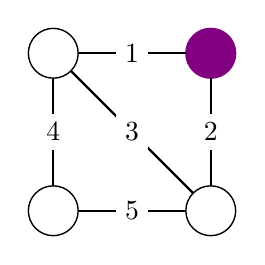
\begin{tikzpicture}[scale=0.5]
	\SetVertexNoLabel
		\Vertex[x=0 ,y=4]{A}
	\begin{scope}[VertexStyle/.append style = {color=violet}]
		\Vertex[x=4 ,y=4]{B}
	\end{scope}
		\Vertex[x=0 ,y=0]{C}
		\Vertex[x=4 ,y=0]{D}
	%	\tikzset{EdgeStyle/.append style = {bend left}}
		\Edge[label = $1$](A)(B)
		\Edge[label = $4$](A)(C)
		\Edge[label = $3$](A)(D)
		\Edge[label = $2$](B)(D)
		\Edge[label = $5$](C)(D)
	\end{tikzpicture}
\end{subfigure}
\begin{subfigure}[b]{0.25\textwidth}
	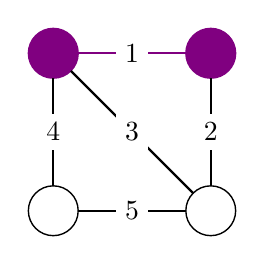
\begin{tikzpicture}[scale=0.5]
	\SetVertexNoLabel
	\begin{scope}[VertexStyle/.append style = {color=violet}]
		\Vertex[x=0 ,y=4]{A}
		\Vertex[x=4 ,y=4]{B}
	\end{scope}
		\Vertex[x=0 ,y=0]{C}
		\Vertex[x=4 ,y=0]{D}
	%	\tikzset{EdgeStyle/.append style = {bend left}}
		\Edge[label = $1$, color=violet](A)(B)
		\Edge[label = $4$](A)(C)
		\Edge[label = $3$](A)(D)
		\Edge[label = $2$](B)(D)
		\Edge[label = $5$](C)(D)
	\end{tikzpicture}
\end{subfigure}
\begin{subfigure}[b]{0.25\textwidth}
	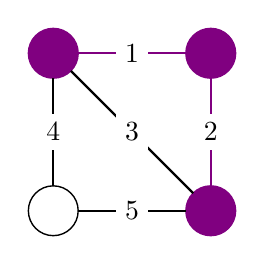
\begin{tikzpicture}[scale=0.5]
	\SetVertexNoLabel
	\begin{scope}[VertexStyle/.append style = {color=violet}]
		\Vertex[x=0 ,y=4]{A}
		\Vertex[x=4 ,y=4]{B}
	\end{scope}
		\Vertex[x=0 ,y=0]{C}
	\begin{scope}[VertexStyle/.append style = {color=violet}]
		\Vertex[x=4 ,y=0]{D}
	\end{scope}
	%	\tikzset{EdgeStyle/.append style = {bend left}}
		\Edge[label = $1$, color=violet](A)(B)
		\Edge[label = $4$](A)(C)
		\Edge[label = $3$](A)(D)
		\Edge[label = $2$, color=violet](B)(D)
		\Edge[label = $5$](C)(D)
	\end{tikzpicture}
\end{subfigure}
\begin{subfigure}[b]{0.20\textwidth}
	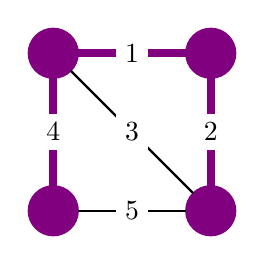
\begin{tikzpicture}[scale=0.5]
	\SetVertexNoLabel
	\begin{scope}[VertexStyle/.append style = {color=violet}]
		\Vertex[x=0 ,y=4]{A}
		\Vertex[x=4 ,y=4]{B}
		\Vertex[x=0 ,y=0]{C}
		\Vertex[x=4 ,y=0]{D}
	\end{scope}
	%	\tikzset{EdgeStyle/.append style = {bend left}}
		\Edge[label = $1$, lw=3pt, color=violet](A)(B)
		\Edge[label = $4$, lw=3pt, color=violet](A)(C)
		\Edge[label = $3$](A)(D)
		\Edge[label = $2$, lw=3pt, color=violet](B)(D)
		\Edge[label = $5$](C)(D)
	\end{tikzpicture}
\end{subfigure}
\end{figure}

Prim`s MST Algorithm pseudo-code:
\begin{itemize}
\item initialize $X=[s]$, $s \in V$ chosen arbitrarily
\item $T =\varnothing$ [invariant: X = vertices spanned by tree-so-far T]
\item while $X \neq V$:
	\begin{itemize}
		\item let $e = (u,v)$ be the cheapest edge of G with $u \in X$, $v \notin X$ 
		\item add e to T
		\item add v to X
	\end{itemize}
	i.e., increasing $\#$ of spanned vertices in cheapest way possible
\end{itemize}



\subsection{MST: Prim`s algorithm correctness proof}
\begin{theorem}Prim`s algorithm always computes an MST. [by two claims]\end{theorem}

\begin{definition} a \underline{cut} of a graph $G=(V,E)$ is a partition of V into 2 non-empty sets (there`s $2^{n-1}$ possible cuts in graph)\end{definition} 

\begin{lemma}[\textbf{empty cut lemma}] a graph is \underline{not} connected $\iff \exists$ cut $(A,B)$ with no crossing edges\end{lemma}
\begin{proof}

\textbf{[$\Leftarrow$]:} assume the RHS. Pick any $u \in A$ and $v \in B$.

Since no edges cross (A,B), there is no u-v path in G $\Rightarrow$ G not connected

\textbf{[$\Rightarrow$]:} assume the LHS. Suppose G has no u-v path.

Define A = {vertices reachable from u in G} [u`s connected components].

Define B = {all other vertices}.

Note: no edges cross the cut (A,B), otherwise A would be bigger)
\end{proof}

\begin{lemma}[\textbf{double-crossing lemma}] suppose the cycle $C \subseteq E$ has an edge crossing the cut (A,B) then so does some other edge of C (at least twice, even number in general)\end{lemma}

\begin{corollary}[\textbf{lonely cut corollary}] if e is the only edge crossing some cut (A,B), then it is not in any cycle.\end{corollary}

\begin{claim} Prim`s algorithm outputs a spanning tree\end{claim}
\begin{proof}
\begin{enumerate}
	\item algorithm maintains invariant that T spans X [by straightforward induction]
	\item can`t get stuck with $X \neq V$ (otherwise the cut (X,V-X) must be empty, by Empty-cut lemma input graph G is disconnected)
	\item no cycles ever get created in T (by lonely cut corollary - we add edge, that first crosses X and V-X - no way to create cycle)
\end{enumerate}
\end{proof}

[MST is unique if edge costs are distinct]

\begin{claim}
\textbf{Cut property}: consider an edge $e$ of $G$. Suppose there is a cut $(A,B)$ such that $e$ is the cheapest edge of $G$ that crosses it. Then $e$ belongs to the MST of $G$.
\end{claim}
\begin{proof}
Will argue by contradiction using an exchange argument [like in scheduling application]

Suppose there is an edge $e$ that is the cheapest one crossing a cut $(A,B)$, yet $e$ is not in the MST $T^*$

\underline{idea:} exchange $e$ with another edge in $T^*$ to make it even cheaper (contradiction)

\underline{note:} since $T^*$ is connected, must contain an edge $f (\neq e)$ crossing (A,B) [by cut lemma]

idea: exchange $e$ and $f$ ($f \in T^*$) to get a spanning tree cheaper than $T^*$ (contradiction) - it may work and may not work, we should exchange correct edge\dots

\underline{hope:} can always find suitable edge $e^`$ so that exchange yields bona fide spanning tree of G

let C = cycle created by adding $e$ to $T^*$

\underline{by double-crossing lemma}: some other edge $e^`$ of C [with $e^` \neq e$ and $e^` \in T^*$] crosses (A,B)

\begin{example}: $T = T^* \cup {e} - {e^`}$ is also a spanning tree\end{example}

Since $c_e < c_{e^`}$, $T$ cheaper than purported MST $T^*$	, contradictioin
\end{proof}

\begin{claim} Cut property $\Rightarrow$ Prim`s algorithm is correct\end{claim}
\begin{proof}
Prim`s algorithm outputs a spanning tree $T^*$ (by previous claim)

\underline{Key point:} Every edge $e \in T^*$ is explicitly justified by the Cut property

$\Rightarrow T^*$ is a subset of the MST

$\Rightarrow$ since $T^*$ is already a spanning tree, it must be the MST
\end{proof}



\subsection{MST: Prim`s algorithm fast implementation}
\begin{itemize}
	\item $O(n)$ iterations
	\item $O(m)$ time per iteration
	\item \textbf{$\Rightarrow O(mn)$ time}
\end{itemize}

\begin{example}use heap to store edges, with keys $=$ edge costs. This leads to $O(m \log n)$ implementation of Prim`s algorithm\end{example}

\begin{invariant}elements in heap $=$ vertices of $V-X$\end{invariant}
\begin{invariant}for $v \in V-X, key[v] =$ cheapest edge $(u,v)$ with $v \in X$ (or $+\infty$ if no such edge exist)\end{invariant}

\begin{example}can initiate heap with $O(m+n \log n) = O(m \log n)$ preprocessing ($O(m)$ to compute keys, $O(n \log n)$ for $n-1$ inserts, $m \geq n-1$ since G is connected)\\\end{example}

\underline{note}: given invariants Extract-min yields next vertex $v \notin V$ and edge $(u,v)$ crossing $(X,V-X)$ to add to X and T respectively
\\

Might need to recompute some keys to maintain Invariant2 after each Extract-min, \underline{pseudocode}:
\begin{itemize}
\item when $v$ added to $X$
\item for each edge $(v,w) \in E$
	\begin{itemize}
		\item if $w \in V-X$
		[the only vertices whose key might have dropped]
		\begin{itemize}
			\item delete $w$ from heap
			[subtle exercise - delete from heap]
			\item recompute $key[w]:= min[key[w],c_vw]$
			\item re-Insert $w$ into heap
		\end{itemize}
		[update key if needed]\\
	\end{itemize}
\end{itemize}

Heap-based implementation:
\begin{itemize}
	\item dominated by time required for heap operations
	\item $n-1$ Inserts during preprocessing
	\item $n-1$ Extract-mins (one per iteration of while loop)
	\item each edge $(v,w)$ triggers one Delete/Insert combo (when it`s first end point gets sucked into X)
	\item $\Rightarrow O(m)$ heap operations (since $m \geq n-1$ as G is connected)
	\item \textbf{$\Rightarrow O(m \log n)$ time}
\end{itemize}



\subsection{MST: Kruskal`s algorithm}
Example:
\begin{figure}[!ht]
\begin{subfigure}[b]{0.25\textwidth}
	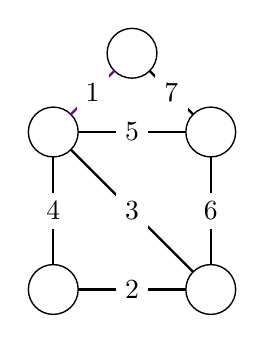
\begin{tikzpicture}[scale=0.5]
	\SetVertexNoLabel
		\Vertex[x=0 ,y=4]{A}
		\Vertex[x=4 ,y=4]{B}
		\Vertex[x=0 ,y=0]{C}
		\Vertex[x=4 ,y=0]{D}
		\Vertex[x=2 ,y=6]{E}
	%	\tikzset{EdgeStyle/.append style = {bend left}}
		\Edge[label = $5$](A)(B)
		\Edge[label = $4$](A)(C)
		\Edge[label = $3$](A)(D)
		\Edge[label = $6$](B)(D)
		\Edge[label = $2$](C)(D)
		\Edge[label = $1$, color=violet](A)(E)		
		\Edge[label = $7$](E)(B)
	\end{tikzpicture}
\end{subfigure}
\begin{subfigure}[b]{0.25\textwidth}
	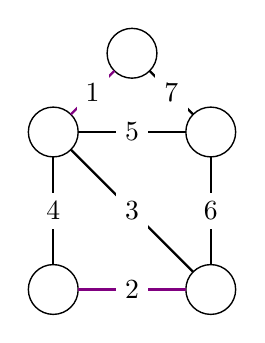
\begin{tikzpicture}[scale=0.5]
	\SetVertexNoLabel
		\Vertex[x=0 ,y=4]{A}
		\Vertex[x=4 ,y=4]{B}
		\Vertex[x=0 ,y=0]{C}
		\Vertex[x=4 ,y=0]{D}
		\Vertex[x=2 ,y=6]{E}
	%	\tikzset{EdgeStyle/.append style = {bend left}}
		\Edge[label = $5$](A)(B)
		\Edge[label = $4$](A)(C)
		\Edge[label = $3$](A)(D)
		\Edge[label = $6$](B)(D)
		\Edge[label = $2$, color=violet](C)(D)
		\Edge[label = $1$, color=violet](A)(E)		
		\Edge[label = $7$](E)(B)
	\end{tikzpicture}
\end{subfigure}
\begin{subfigure}[b]{0.25\textwidth}
	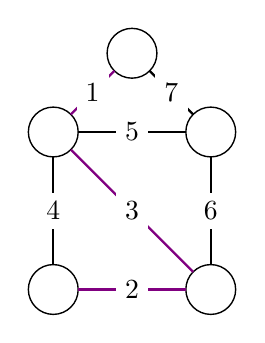
\begin{tikzpicture}[scale=0.5]
	\SetVertexNoLabel
		\Vertex[x=0 ,y=4]{A}
		\Vertex[x=4 ,y=4]{B}
		\Vertex[x=0 ,y=0]{C}
		\Vertex[x=4 ,y=0]{D}
		\Vertex[x=2 ,y=6]{E}
	%	\tikzset{EdgeStyle/.append style = {bend left}}
		\Edge[label = $5$](A)(B)
		\Edge[label = $4$](A)(C)
		\Edge[label = $3$, color=violet](A)(D)
		\Edge[label = $6$](B)(D)
		\Edge[label = $2$, color=violet](C)(D)
		\Edge[label = $1$, color=violet](A)(E)		
		\Edge[label = $7$](E)(B)
	\end{tikzpicture}
\end{subfigure}
\begin{subfigure}[b]{0.25\textwidth}
	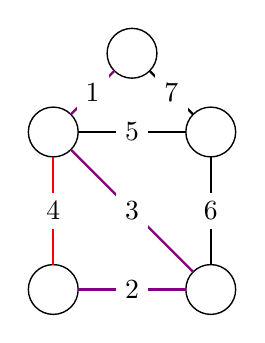
\begin{tikzpicture}[scale=0.5]
	\SetVertexNoLabel
		\Vertex[x=0 ,y=4]{A}
		\Vertex[x=4 ,y=4]{B}
		\Vertex[x=0 ,y=0]{C}
		\Vertex[x=4 ,y=0]{D}
		\Vertex[x=2 ,y=6]{E}
	%	\tikzset{EdgeStyle/.append style = {bend left}}
		\Edge[label = $5$](A)(B)
		\Edge[label = $4$, color=red](A)(C)
		\Edge[label = $3$, color=violet](A)(D)
		\Edge[label = $6$](B)(D)
		\Edge[label = $2$, color=violet](C)(D)
		\Edge[label = $1$, color=violet](A)(E)		
		\Edge[label = $7$](E)(B)
	\end{tikzpicture}
\end{subfigure}
\begin{subfigure}[b]{0.25\textwidth}
	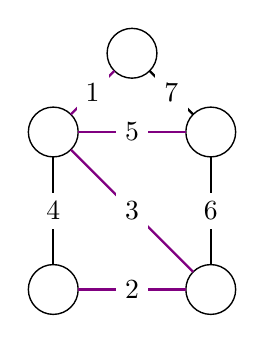
\begin{tikzpicture}[scale=0.5]
	\SetVertexNoLabel
		\Vertex[x=0 ,y=4]{A}
		\Vertex[x=4 ,y=4]{B}
		\Vertex[x=0 ,y=0]{C}
		\Vertex[x=4 ,y=0]{D}
		\Vertex[x=2 ,y=6]{E}
	%	\tikzset{EdgeStyle/.append style = {bend left}}
		\Edge[label = $5$, color=violet](A)(B)
		\Edge[label = $4$](A)(C)
		\Edge[label = $3$, color=violet](A)(D)
		\Edge[label = $6$](B)(D)
		\Edge[label = $2$, color=violet](C)(D)
		\Edge[label = $1$, color=violet](A)(E)		
		\Edge[label = $7$](E)(B)
	\end{tikzpicture}
\end{subfigure}
\begin{subfigure}[b]{0.25\textwidth}
	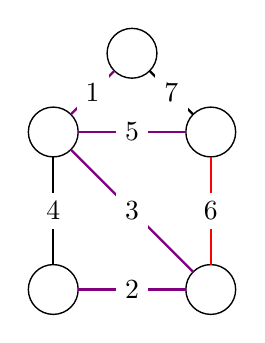
\begin{tikzpicture}[scale=0.5]
	\SetVertexNoLabel
		\Vertex[x=0 ,y=4]{A}
		\Vertex[x=4 ,y=4]{B}
		\Vertex[x=0 ,y=0]{C}
		\Vertex[x=4 ,y=0]{D}
		\Vertex[x=2 ,y=6]{E}
	%	\tikzset{EdgeStyle/.append style = {bend left}}
		\Edge[label = $5$, color=violet](A)(B)
		\Edge[label = $4$](A)(C)
		\Edge[label = $3$, color=violet](A)(D)
		\Edge[label = $6$, color=red](B)(D)
		\Edge[label = $2$, color=violet](C)(D)
		\Edge[label = $1$, color=violet](A)(E)		
		\Edge[label = $7$](E)(B)
	\end{tikzpicture}
\end{subfigure}
\begin{subfigure}[b]{0.25\textwidth}
	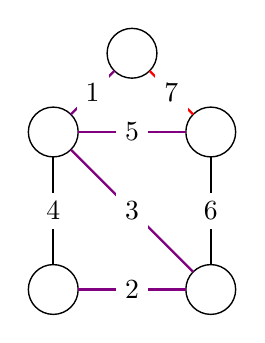
\begin{tikzpicture}[scale=0.5]
	\SetVertexNoLabel
		\Vertex[x=0 ,y=4]{A}
		\Vertex[x=4 ,y=4]{B}
		\Vertex[x=0 ,y=0]{C}
		\Vertex[x=4 ,y=0]{D}
		\Vertex[x=2 ,y=6]{E}
	%	\tikzset{EdgeStyle/.append style = {bend left}}
		\Edge[label = $5$, color=violet](A)(B)
		\Edge[label = $4$](A)(C)
		\Edge[label = $3$, color=violet](A)(D)
		\Edge[label = $6$](B)(D)
		\Edge[label = $2$, color=violet](C)(D)
		\Edge[label = $1$, color=violet](A)(E)		
		\Edge[label = $7$, color=red](E)(B)
	\end{tikzpicture}
\end{subfigure}
\end{figure}

\begin{figure}[!ht]
\begin{subfigure}[b]{\textwidth}
	\begin{center}
	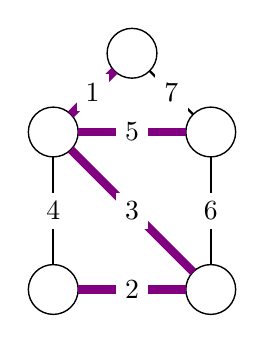
\begin{tikzpicture}[scale=0.5]
	\SetVertexNoLabel
		\Vertex[x=0 ,y=4]{A}
		\Vertex[x=4 ,y=4]{B}
		\Vertex[x=0 ,y=0]{C}
		\Vertex[x=4 ,y=0]{D}
		\Vertex[x=2 ,y=6]{E}
	%	\tikzset{EdgeStyle/.append style = {bend left}}
		\Edge[label = $5$, lw=3pt, color=violet](A)(B)
		\Edge[label = $4$](A)(C)
		\Edge[label = $3$, lw=3pt, color=violet](A)(D)
		\Edge[label = $6$](B)(D)
		\Edge[label = $2$, lw=3pt, color=violet](C)(D)
		\Edge[label = $1$, lw=3pt, color=violet](A)(E)		
		\Edge[label = $7$](E)(B)
	\end{tikzpicture}
	\end{center}
\end{subfigure}
\end{figure}

Kruskal`s MST Algorithm pseudo-code:
\begin{itemize}
\item sort edges in order of increasing cost [rename edges 1,2,3,\dots,m so that $c_1 < c_2 < \dots < c_m$]
\item $T =\varnothing$
\item for $i = 1$ to $m$
	\begin{itemize}
		\item if $T \cup [i]$ has no cycles
		\begin{itemize}
			\item add i to T
		\end{itemize}
	\end{itemize}
\item return T
\end{itemize}



\subsection{MST: Kruskal`s algorithm correctness proof}
\begin{theorem}Kruskal`s algorithm is correct\end{theorem}

\begin{proof}
Let $T^* =$ output of Kruskal`s algorithm on input graph G
\begin{enumerate}
	\item clearly $T^*$ has no cycles (by algorithm itself)
	\item $T^*$ is connected because:
	\begin{enumerate}
		\item by empty-cut lemma, only need to show that $T^*$ crosses every cut
		\item fix a cut $(A, B)$. Since $G$ connected at least one of its edges crosses $(A, B)$
		\textbf{Key point}: Kruskal`s algorithm will include first edge crossing $(A, B)$ that it sees [by lonely-cut corollary, cannot create a cycle]
	\end{enumerate}
	$\Rightarrow$ Kruskal`s algorithm outputs a spanning tree
	\item every edge of $T^*$ justified by the Cut Property (implies $T^*$ is the MST)
	\begin{enumerate}
		\item consider iteration where edge $(u, v)$ added to current set $T$ (some current state of Kruskal`s algorithm). Since $T \cup [(u, v)]$ has no cycle, T has no u-v path
		
		$\Rightarrow \exists$ empty cut $(A, B)$ separating $u$ and $v$
		
		$\Rightarrow$ by previous $2b$, no edges crossing $(A, B)$ were previously considered by Kruskal`s algorithm
		
		$\Rightarrow$ $(u, v)$ is the first (and cheapest) edge crossing $(A, B)$
		
		$\Rightarrow$ $(u, v)$ justified by the Cut Property
	\end{enumerate}
\end{enumerate}
\end{proof}



\subsection{MST: Kruskal`s algorithm via Union-Find}
Running time of straightforward implementation:
\begin{itemize}
	\item $O(m \log n)$ for sorting edges (recall $m = O(n^2)$, no parallel edges)
	\item $m$ iterations
	\item $O(n)$ to check cycles (search for other path with BFS or DFS in graph $(V, T)$, $\leq (n-1)$ edges)
	\item $\Rightarrow O(m \log n) + O(mn) = O(mn)$\\
\end{itemize}

Plan: data structure for $O(1)$-time cycle checks? $\Rightarrow O(m \log n)$
\\

Union-find data structures:
\begin{itemize}
	\item maintain partition of a set of objects
	\item $FIND(x)$: return name of a group that $x$ belongs to
	\item $UNION(c_i, c_j)$: fuse groups $c_i$ and $c_j$ into a single one.\\
\end{itemize}

For Kruskal algorithm:
\begin{itemize}
	\item objects $=$ vertices
	\item groups $=$ connected components with currently chosen edges $T$
	\item adding new edge $(u, v)$ to $T$ $\iff$ fusing connected components of $u, v$
\end{itemize}

\begin{enumerate}
	\item \textbf{Idea1}:
	\begin{itemize}
		\item maintain one linked structure per connected component of $(V, T)$
		\item each component has an arbitrary \underline{leader} vertex
		\item \textbf{Invariant}: each vertex points to the leader of its component ["name" of a component inherited from leader vertex]
		\item \textbf{Key point}: given edge $(u, v)$, can check if $u|v$ already in same component in $O(1)$ time [$\iff$ leader pointers match, $FIND(u) = FIND(v)$]
		\item $\Rightarrow O(1)$-time cycle checks!
		\item Maintaining the invariant: when new edge $(u, v)$ added to $T$, connected components of $u|v$ merge [at most $\theta(n)$ operations with pointers \underline{each time}]
	\end{itemize}
	\item \textbf{Idea2}:
	\begin{itemize}
		\item when two components merge, have smaller one inherit the leader of the larger one [maintain a size field in each component]
		\item $\theta(n)$ worst case updates to restore invariant
		\item single vertex can have $\theta(\log_2 n)$ pointers update over the courser of Kruskal`s algorithm [at each update population at least doubles]
	\end{itemize}
\end{enumerate}

Running time of fast implementation:
\begin{itemize}
	\item $O(m \log n)$ time for sorting
	\item $O(m)$ time for cycle checks [$O(1)$ per iteration]
	\item $O(n \log n)$ time overall for leader pointer updates
	\item $\Rightarrow O(m \log n)$ total running time
\end{itemize}



\subsection{MST: State of art and Open questions}
\textbf{Question}: can we do better than $O(m \log n)$ (running tyme for Prims or Kruskal algorithms)?

\underline{Answer: yes!}
\begin{itemize}
	\item randomized algorithm with $O(m)$ running time [Karger-Klein-Tarjan JACM 1995]
	\item deterministic algorithm with $O(m \alpha(n))$ running time [Chazelle JACM 2000], $\alpha(n) =$ "inverse Ackermann function" - in particular, grows much slower than $\log^* n :=$ number of times you can apply $\log$ to $n$ until result drops below $1$ (inverse of "tower function" $2^{2^{...^{2}}}$)
\end{itemize}

\underline{Open questions}:
\begin{enumerate}
	\item \textbf{Weirdest of all}: [Pettie/Ramachandran JACM 2002] optimal deterministic MST algorithm, but precise asymptotic running time is \underline{unknown}! (somewhere between $\Theta(m)$ and $\Theta(m \alpha(n))$)
	\item simple randomized $O(m)$-time algorithm for MST (sufficient: do this just for the "MST-verification" problem)
	\item is there a deterministic $O(m)$-time algorithm?
\end{enumerate}

Further reading - [Eisner, 1997]



\subsection{MST: Application to clustering}
\textbf{Informal goal}: given $n$ "points" [web pages, images, genome fragments, etc] classify into "coherent groups"
\\

\textbf{Assumption}:
\begin{description}
	\item{(1)} as input, given a (dis)similarity measure - a distance $d(p, q)$ between each point pair
	\item{(2)} symmetric [i.e., $d(p, q) = d(q, p)$]
\end{description}

\begin{example}Euclidean distance, genome similarity, etc.\\\end{example}


\textbf{Goal}: Same cluster $\iff$ "nearby"
\\

\textbf{[Assume]:} we know k$:= \#$ of clusters desired [in practice, can experiment with a range of values]
\\

\begin{definition} call points $p|q$ \underline{separated} if they`re assigned to different clusters\end{definition}
\begin{definition} the \underline{spacing} of a $k$-clustering is $\min\limits_{p,q-separated} d(p, q)$ [the bigger, the better]\end{definition}

\textbf{[Problem statement]:} given a distance measure d and k, compute the k-clustering with maximum spacing
\\

\textbf{Single-link clustering} pseudo-code [just like Kruskal`s MST algorithm, \underline{but stopped earlier}]:
\begin{itemize}
\item initially, each point in a separate cluster
\item repeat until only k clusters:
	\begin{itemize}
		\item let $p, q =$ closest pair of separated points (determines the current spacing)
		\item merge the clusters containing $p|q$ into a single cluster
	\end{itemize}
\end{itemize}

\begin{theorem}single-link clustering finds the $\max$-spacing $k$-clustering\end{theorem}

\begin{proof}
Let $C_1, \dots, C_k =$ greedy clustering with spacing $S$

Let $\widehat{C_1}, \dots, \widehat{C_k} =$ arbitrary other clustering

\textbf{Need to show}: spacing of $\widehat{C_1}, \dots \widehat{C_k} \leq S$

\begin{case}$\widehat{C_i}$`s are the same as the $C_i$`s [may be after renaming] $\Rightarrow$ has the same spacing S\end{case}
\begin{case}
otherwise, can find a point pair $p, q$ such that
\begin{description}
	\item{(A)} $p, q$ in the same greedy cluster $C_i$
	\item{(B)} $p, q$ in different clusters $\widehat{C_i}, \widehat{C_j}$
\end{description}

\textbf{Property of greedy algorithm}: if two points $x, y$ "directly merged" at some point, then $d(x, y) \leq S$ [distance between merged point pairs only goes up]

\begin{description}
	\item{(Easy case)} if $p, q$ directly merged at some point, $S \geq d(p, q) \geq$ spacing of $\widehat{C_1}, \dots, \widehat{C_k}$
	\item{(Tricky case)} $p, q$ "indirectly merged" through multiple direct merges.

	Let $p, a_1, \dots, a_l, q$ be the path of direct greedy merges connecting $p|a$

	\textbf{Key point}: since $p \in \widehat{C_i}$ and $q \notin \widehat{C_i}$, $\exists$ consecutive pair $a_j, a_{j+1}$ with $a_j \in \widehat{C_i}, a_{j+1} \notin \widehat{C_i}$

	$\Rightarrow S \geq d(a_j, a_{j+1})$ [since $a_j, a_{j+1}$ directly merged] $\geq$ spacing of $\widehat{C_1}, \dots, \widehat{C_k}$ [since $a_j, a_{j+1}$ separated]
\end{description}

\end{case}
\end{proof}



\subsection{Huffman codes}
\begin{definition}\underline{Binary code}: maps each character of an alphabet $\Sigma$ to a binary string\end{definition}
\begin{example}$\Sigma = a-z$ various punctuation (size $32$ overall say)\end{example}
\begin{example}\textbf{Obvious encoding} --- use the 32 5-bit binary strings to encode this $\Sigma$ (a fixed length code)\end{example}

\underline{We can do better} if some characters of $\Sigma$ are much more frequent than others, using a variable-length code.
\\

\begin{example}Suppose $\Sigma = \{A, B, C, D\}$, fixed-length encoding would be $\{00, 01, 10, 11\}$\end{example}
\begin{example}Suppose instead we use the encoding $\{0, 01, 10, 1\}$ - not enough information in encoding $001$\end{example}

\textbf{[Problem]:} with variable-length codex, not clear where one character ends and the next one begins
\\

\textbf{[Solution]:} \underline{prefix-free codes} --- make sure that for every paif $i, j \in \Sigma$, neither of the encodings $f(i), f(j)$ is a prefix of the other.
\\

\begin{example}$\{0, 10, 11, 111\}$ --- correct variable-length prefix-free encoding\end{example}
\begin{example}$A - 60~\%$, $B - 25~\%$, $C - 10~\%$, $D - 5~\%$. For fixed-length encoding -- $2$ bits/character, for variable-length encoding $\{{0, 10, 110, 111}\}$ -- $1.55$ bits/character on average\end{example}

\textbf{[Goal]:} best binary prefix-free encoding for a given set of character frequencies
\\

\textbf{[Useful fact]:} binary codes $\iff$ binary trees
\\

\begin{example}$\Sigma = \{A, B, C, D\}$
\begin{figure}[!ht]
\begin{subfigure}[b]{0.4\textwidth}
	$\{00, 01, 10, 11\}$\\
	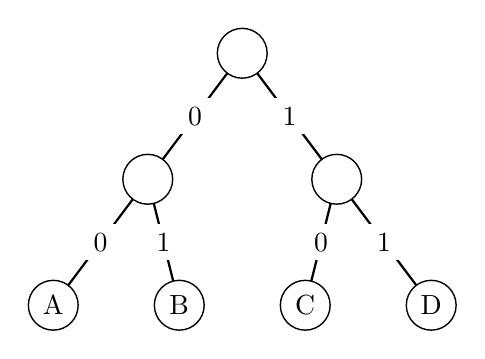
\begin{tikzpicture}[scale=0.4]
		\Vertex[x=0 ,y=0]{A}
		\Vertex[x=4 ,y=0]{B}
		\Vertex[x=8 ,y=0]{C}
		\Vertex[x=12 ,y=0]{D}
	\SetVertexNoLabel
		\Vertex[x=3 ,y=4]{E}
		\Vertex[x=9 ,y=4]{F}
		\Vertex[x=6 ,y=8]{root}
	%	\tikzset{EdgeStyle/.append style = {bend left}}
		\Edge[label = $0$](E)(A)
		\Edge[label = $1$](E)(B)
		\Edge[label = $0$](F)(C)
		\Edge[label = $1$](F)(D)
		\Edge[label = $0$](root)(E)
		\Edge[label = $1$](root)(F)
	\end{tikzpicture}
\end{subfigure}
\begin{subfigure}[b]{0.25\textwidth}
	$\{0, 01, 10, 1\}$\\
	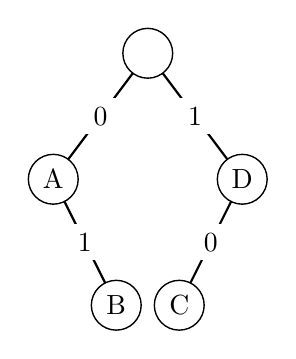
\begin{tikzpicture}[scale=0.4]
		\Vertex[x=3 ,y=4]{A}
		\Vertex[x=5 ,y=0]{B}
		\Vertex[x=7 ,y=0]{C}
		\Vertex[x=9 ,y=4]{D}
	\SetVertexNoLabel
		\Vertex[x=6 ,y=8]{root}
	%	\tikzset{EdgeStyle/.append style = {bend left}}
		\Edge[label = $1$](A)(B)
		\Edge[label = $0$](D)(C)
		\Edge[label = $0$](root)(A)
		\Edge[label = $1$](root)(D)
	\end{tikzpicture}
\end{subfigure}
\begin{subfigure}[b]{0.25\textwidth}
	$\{0, 10, 110, 111\}$ -- labels only at the leaves\\
	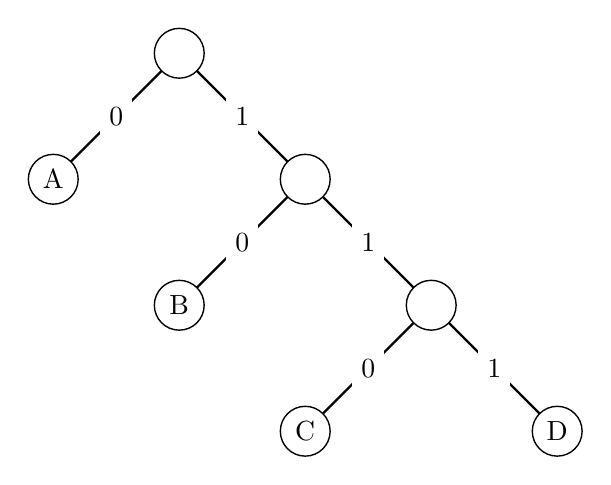
\begin{tikzpicture}[scale=0.4]
		\Vertex[x=0 ,y=8]{A}
		\Vertex[x=4 ,y=4]{B}
		\Vertex[x=8 ,y=0]{C}
		\Vertex[x=16 ,y=0]{D}
	\SetVertexNoLabel
		\Vertex[x=4 ,y=12]{root}
		\Vertex[x=8 ,y=8]{subroot1}
		\Vertex[x=12 ,y=4]{subroot2}
	%	\tikzset{EdgeStyle/.append style = {bend left}}
		\Edge[label = $0$](root)(A)
		\Edge[label = $1$](root)(subroot1)
		\Edge[label = $0$](subroot1)(B)
		\Edge[label = $1$](subroot1)(subroot2)
		\Edge[label = $0$](subroot2)(C)
		\Edge[label = $1$](subroot2)(D)
	\end{tikzpicture}
\end{subfigure}
\end{figure}

\end{example}

\textbf{[In general]:} left child edges $\iff "0"$, right child edges $\iff "1"$
\begin{itemize}
	\item for each $i \in \Sigma$, exactly one node labeled $"i"$
	\item encoding of $i \in \Sigma \iff$ bits along path from root to the node
	\item prefix-free $\iff$ labelled nodes $=$ the leaves [since prefixes $\iff$ one node an ancestor of another]
\end{itemize}

\textbf{[To decode]:} repeatedly follow path from root until you hit a leaf (unambigous since only leaves are labelled)
\\

\textbf{[Note]:} encoding length of $i \in \Sigma =$ depth of $i$ in tree
\\

\textbf{[Problem]:} input -- probability $p_i$ for each character $i \in \Sigma$. Output -- a binary tree $T$ minimizing the average encoding length $L()$

\begin{definition}if $T =$ tree with leaves $\iff$ symbols of $\Sigma$, then average encoding length $L(T) = \sum\limits_{i \in \Sigma} p_i*$[depth of i in T]\end{definition}

\textbf{Natural idea}: top down / divide and conquer (partition $\Sigma$ into two, with $50~\%$ of total frequency)

\textbf{Huffman`s (optional) idea}: build tree \underline{bottom-up} using successive mergers

\begin{observation}final encoding length of $i \in \Sigma = \#$ of mergers its subtree endures\end{observation}

\begin{figure}[ht!]
\begin{subfigure}[b]{0.5\textwidth}
	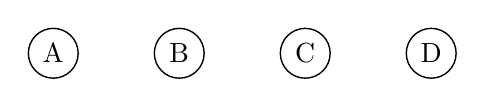
\begin{tikzpicture}[scale=0.4]
		\Vertex[x=0 ,y=0]{A}
		\Vertex[x=4 ,y=0]{B}
		\Vertex[x=8 ,y=0]{C}
		\Vertex[x=12 ,y=0]{D}
	\end{tikzpicture}
\end{subfigure}
\begin{subfigure}[b]{0.5\textwidth}
	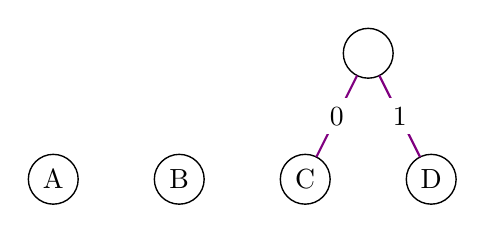
\begin{tikzpicture}[scale=0.4]
		\Vertex[x=0 ,y=0]{A}
		\Vertex[x=4 ,y=0]{B}
		\Vertex[x=8 ,y=0]{C}
		\Vertex[x=12 ,y=0]{D}
		\SetVertexNoLabel
		\Vertex[x=10 ,y=4]{subroot2}
	%	\tikzset{EdgeStyle/.append style = {bend left}}
		\Edge[label = $0$, color=violet](subroot2)(C)
		\Edge[label = $1$, color=violet](subroot2)(D)
	\end{tikzpicture}
\end{subfigure}
\begin{subfigure}[b]{0.5\textwidth}
	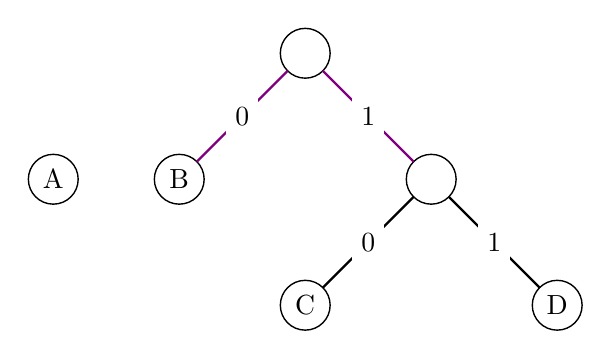
\begin{tikzpicture}[scale=0.4]
		\Vertex[x=0 ,y=4]{A}
		\Vertex[x=4 ,y=4]{B}
		\Vertex[x=8 ,y=0]{C}
		\Vertex[x=16 ,y=0]{D}
		\SetVertexNoLabel
		\Vertex[x=8 ,y=8]{subroot1}
		\Vertex[x=12 ,y=4]{subroot2}
	%	\tikzset{EdgeStyle/.append style = {bend left}}
		\Edge[label = $0$, color=violet](subroot1)(B)
		\Edge[label = $1$, color=violet](subroot1)(subroot2)
		\Edge[label = $0$](subroot2)(C)
		\Edge[label = $1$](subroot2)(D)
	\end{tikzpicture}
\end{subfigure}
\begin{subfigure}[b]{0.5\textwidth}
	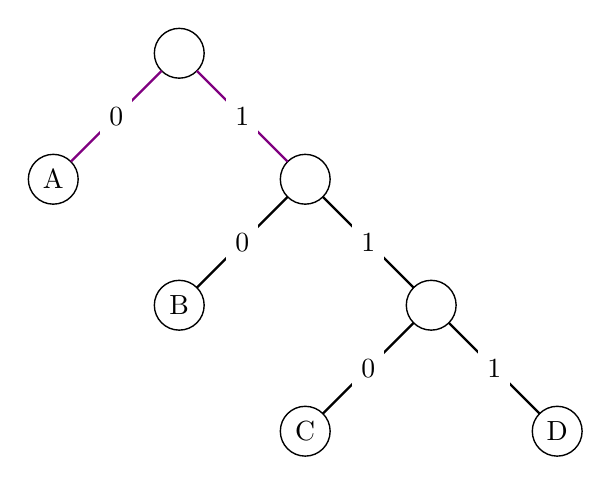
\begin{tikzpicture}[scale=0.4]
		\Vertex[x=0 ,y=8]{A}
		\Vertex[x=4 ,y=4]{B}
		\Vertex[x=8 ,y=0]{C}
		\Vertex[x=16 ,y=0]{D}
		\SetVertexNoLabel
		\Vertex[x=4 ,y=12]{root}
		\Vertex[x=8 ,y=8]{subroot1}
		\Vertex[x=12 ,y=4]{subroot2}
	%	\tikzset{EdgeStyle/.append style = {bend left}}
		\Edge[label = $0$, color=violet](root)(A)
		\Edge[label = $1$, color=violet](root)(subroot1)
		\Edge[label = $0$](subroot1)(B)
		\Edge[label = $1$](subroot1)(subroot2)
		\Edge[label = $0$](subroot2)(C)
		\Edge[label = $1$](subroot2)(D)
	\end{tikzpicture}
\end{subfigure}
\end{figure}

\textbf{Huffman`s algorithm}:
\begin{itemize}
	\item if $|\Sigma| = 2$ return (1)
	\item let $a, b \in \Sigma$ have \underline{the smallest frequences}
	\item let $\Sigma^` = \Sigma$ with $a, b$ replaced by new symbol $ab$
	\item define $p_{ab} = p_a + p_b$
	\item recursively compute $T^`$ (for the alphabet $\Sigma^`$)
	\item extend $T^`$ (with leaves $\iff \Sigma^`$) to a tree $T$ with leaves $\iff \Sigma$ by splitting leaf $ab$ into two leaves $a|b$
	\item return $T$
\end{itemize}

\begin{figure}[ht!]
\begin{subfigure}[b]{0.5\textwidth}
	(1)
	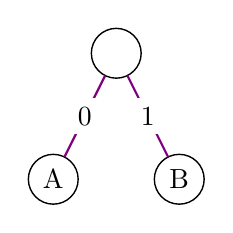
\begin{tikzpicture}[scale=0.4]
		\Vertex[x=0 ,y=0]{A}
		\Vertex[x=4 ,y=0]{B}
		\SetVertexNoLabel
		\Vertex[x=2 ,y=4]{subroot2}
	%	\tikzset{EdgeStyle/.append style = {bend left}}
		\Edge[label = $0$, color=violet](subroot2)(A)
		\Edge[label = $1$, color=violet](subroot2)(B)
	\end{tikzpicture}
\end{subfigure}
\end{figure}

\begin{theorem} [Huffman, 52] Huffman`s algorithm computes a binary tree (with leaves $\iff$ symbols of $\Sigma$) that minimizes the average encoding length\end{theorem}

\begin{proof}
By induction on $n = |\Sigma|$ (can assume $n \geq 2$)
\begin{description}
	\item{(base case)} when $n = 2$, algoruthm outputs the optimal tree (1) - 1 bit per symbol
	\item{(induction hypothesis)} algorithm solves smaller subproblem optimally (for $\Sigma^`$) - $\widehat{T^`}$
	\item{(inductive step)} fix input with $n = |\Sigma| > 2$

	Let $\Sigma^` = \Sigma$ with $a, b$ (smallest frequency) replaced by meta-symbol $ab$ ($p_{ab} = p_a + p_b$)

	Exact correspondence $T \iff T^`$. Let trees for $\Sigma$ that have $a, b$ as siblings ($T1$) - $X_{ab}$

	\textbf{important}: for every such pair $T^`$ and $T$, $L(T)-L(T^`) = p_a(d+1) + p_b(d+1) - (p_a+p_b)d = p_a + p_b$ - \textbf{independent of $T, T^`$}

	\textbf{upshot}: corresponding tree $\widehat{T^`}$ minimizes $L(T)$ for $\Sigma$ over all trees in $X_{ab}$ (where $a|b$ are siblings)

	\textbf{key lemma} complete`s proof of theorem
\end{description}
\end{proof}

\begin{lemma}there is an optimal tree (for $\Sigma$) in $X_{ab}$ [i.e. $a, b$ were "safe" to merge]\end{lemma}

\begin{proof}
\textbf{Intuition}: can make an optimal tree better by pushing $a|b$ as deep as possible (since $a, b$ have smallest frequencies)

[By exchange argument]
\\

Let $T^*$ be any tree that minimizes $L(T)$ for $\Sigma$

Let $x, y$ be siblings at the deepest level of $T^*$

\textbf{exchange}: obtain $\widehat{T}$ from $T^*$ by swapping labels $a \leftarrow\rightarrow x, b \leftarrow\rightarrow y$
\\

[note]: $\widehat{T} \in X_{ab}$ by choice of $x, y$
\\

$L(T^*) - L(\widehat{T}) = (p_x-p_a)[$depth of $x$ in $T^* -$ depth of $a$ in $T^*] + (p_y-p_b)[$depth of $y$ in $T^* -$ depth of b in $T^*] \geq 0$, since

$(p_x-p_a), (p_y-p_b) \geq 0$ (smallest frequency of $a,b$) and by choice of $x, y$

$\Rightarrow L(\widehat{T}) \leq L(T^*)$

$\Rightarrow \widehat{T}$ also optimal
\end{proof}

\textbf{Running time}:
\begin{itemize}
	\item \underline{naive implementation} - $O(n^2)$, where $n = |\Sigma|$
	\item \underline{speed ups} use a heap (repeated minimum computations)

	keys - frequences

	after extracting the two smallest-frequency symbols, re-Insert the new meta-symbol [key - sum of the $2$ old one`s]

	$\Rightarrow$ iterative, $O(n \log n)$ implementation
	\item \underline{even faster} sorting + $O(n)$ additional work

	\begin{example}manage (meta-)symbols using two queues\end{example}
\end{itemize}





\newpage
\section{Dynamic programming}



\subsection{Weighted independent sets in path graphs}
\textbf{[Input]:} a path graph $G = (V, E)$ with nonnegative weights on vertices
\\

\textbf{[Desired output]:} subset of nonadjacent vertices - an \underline{independent set} - of maximum total weight
\\

\textbf{Greedy algorithm}: iteratively choose the max-weight vertex not adjacent to any previously chosen vertex
\\

\textbf{Divide and Conquer algorithm}: recursively compute the max-weight IS of the 1st hals, for 2nd hald, then combine the solutions

\begin{figure}[ht!]
\begin{subfigure}[b]{\textwidth}
\begin{center}
	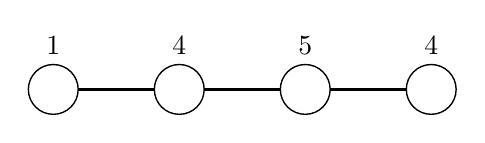
\begin{tikzpicture}[scale=0.4]
		\SetVertexNoLabel
	\begin{scope}[VertexStyle/.append style = {label=$1$}]
		\Vertex[x=4 ,y=0]{A}
	\end{scope}
	\begin{scope}[VertexStyle/.append style = {label=$4$}]
		\Vertex[x=8 ,y=0]{B}
	\end{scope}
	\begin{scope}[VertexStyle/.append style = {label=$5$}]
		\Vertex[x=12 ,y=0]{C}
	\end{scope}
	\begin{scope}[VertexStyle/.append style = {label=$4$}]
		\Vertex[x=16 ,y=0]{D}
	\end{scope}
	%	\tikzset{EdgeStyle/.append style = {bend left}}
		\Edge(A)(B)
		\Edge(B)(C)
		\Edge(C)(D)
	\end{tikzpicture}
\end{center}
\end{subfigure}
\begin{subfigure}[b]{0.5\textwidth}
	Greedy
	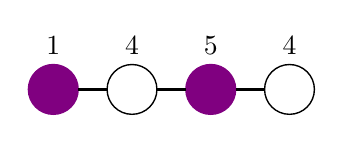
\begin{tikzpicture}[scale=0.25]
		\SetVertexNoLabel
	\begin{scope}[VertexStyle/.append style = {label=$1$, color=violet}]
		\Vertex[x=4 ,y=0]{A}
	\end{scope}
	\begin{scope}[VertexStyle/.append style = {label=$4$}]
		\Vertex[x=8 ,y=0]{B}
	\end{scope}
	\begin{scope}[VertexStyle/.append style = {label=$5$, color=violet}]
		\Vertex[x=12 ,y=0]{C}
	\end{scope}
	\begin{scope}[VertexStyle/.append style = {label=$4$}]
		\Vertex[x=16 ,y=0]{D}
	\end{scope}
	%	\tikzset{EdgeStyle/.append style = {bend left}}
		\Edge(A)(B)
		\Edge(B)(C)
		\Edge(C)(D)
	\end{tikzpicture}
\end{subfigure}
\begin{subfigure}[b]{0.5\textwidth}
	Optimal solution
	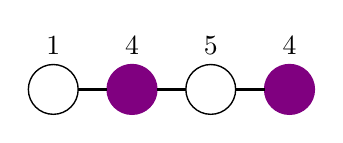
\begin{tikzpicture}[scale=0.25]
		\SetVertexNoLabel
	\begin{scope}[VertexStyle/.append style = {label=$1$}]
		\Vertex[x=4 ,y=0]{A}
	\end{scope}
	\begin{scope}[VertexStyle/.append style = {label=$4$, color=violet}]
		\Vertex[x=8 ,y=0]{B}
	\end{scope}
	\begin{scope}[VertexStyle/.append style = {label=$5$}]
		\Vertex[x=12 ,y=0]{C}
	\end{scope}
	\begin{scope}[VertexStyle/.append style = {label=$4$, color=violet}]
		\Vertex[x=16 ,y=0]{D}
	\end{scope}
	%	\tikzset{EdgeStyle/.append style = {bend left}}
		\Edge(A)(B)
		\Edge(B)(C)
		\Edge(C)(D)
	\end{tikzpicture}
\end{subfigure}
\begin{subfigure}[b]{\textwidth}
	Divide and conquer [conflict]
	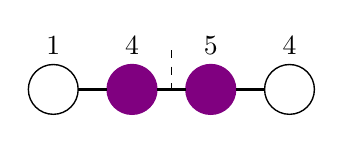
\begin{tikzpicture}[scale=0.25]
		\SetVertexNoLabel
	\begin{scope}[VertexStyle/.append style = {label=$1$}]
		\Vertex[x=4 ,y=0]{A}
	\end{scope}
	\begin{scope}[VertexStyle/.append style = {label=$4$, color=violet}]
		\Vertex[x=8 ,y=0]{B}
	\end{scope}
	\begin{scope}[VertexStyle/.append style = {label=$5$, color=violet}]
		\Vertex[x=12 ,y=0]{C}
	\end{scope}
	\begin{scope}[VertexStyle/.append style = {label=$4$}]
		\Vertex[x=16 ,y=0]{D}
	\end{scope}
	%	\tikzset{EdgeStyle/.append style = {bend left}}
		\Edge(A)(B)
		\Edge(B)(C)
		\Edge(C)(D)
		\draw[dashed] (10,2) -- (10,0);
	\end{tikzpicture}
\end{subfigure}
\end{figure}



\subsection{WIS: optimal substructure}
\textbf{[Critical step]:} reason about structure of an optimal solution (in terms of optimal solution of smaller subproblem)
\\

Motivation - experiment narrows down the set of candidates for the optimal solution (can search through the small set using brute-force-search)
\\

Let $S \subseteq V$ be a max-weight independent set (IS). Let $v_n =$ last vertex of path.
\begin{case}
Suppose $v_n \notin S$. Let $G^` = G$ with $v_n$ deleted.

Note: S also an IS of $G^`$

Note: S must be a max-weight IS of $G^`$ - if $S^*$ was better, it would also be better than $S$ in $G$ [contradiction]
\end{case}
\begin{case}
Suppose $v_n \in S$

note: previous vertex $v_{n-1} \notin S$ [by IS definition]. Let $G^" = G$ with $v_{n-1}, v_n$ deleted

note: $S - \{v_n\}$ is an IS of $G^"$

note: must in fact be a max-weitght IS of $G^"$ -- if $S^*$ is better than S in $G^"$, then $S^* \cup \{v_n\}$ is better than $S$ in $G$ [contradiction] 
\end{case}

\begin{corollary}\underline{if we knew} whether or not $v_n$ was in the max-weight IS, could recursively compute the max-weight IS of $G^`$ or $G^"$ [$G^" +$ $v_n$ weight] and be done\end{corollary}
\textbf{[Crazy idea]:} try both possibilities and return the better solution



\subsection{WIS: linear-time algorithm}
\begin{enumerate}
	\item recursively compute $s_1 =$ max-wt IS of $G^`$
	\item recursively compute $s_2 =$ max-wt IS of $G^"$
	\item return $s_1$ or $s_2 \cup \{v_n\}$, whichever is better
\end{enumerate}
\begin{example} Proof correctness formally by induction\end{example}

\textbf{[Bad news]:} exponential time (like a brute-force)\

But, \underline{only $\Theta(n)$ distinct subproblems} ever get solved by this algorithm
\\

To eliminate redundancy - the first time you solve a subproblem, cache its solution in a global table for $O(1)$-time lookup later ["memoization"]
\\

\textbf{[Even better]:} reformulate as a bottom-up iterative algorithm. Let $G_i =$ 1st $i$ vertices of $G$
\begin{enumerate}
	\item populate array A left to right with $A[i] =$ value of max-wt IS of $G_i$
	\item $A[0] = 0$, $A[1] = w_1$
	\item main loop: for $i = 2, 3, \dots, n: A[i] = max\{A[i-1], A[i-2]+w_i\}$ (case1 and case2)
\end{enumerate}

\textbf{Running time $O(n)$}

Correctness: same as recursive version



\subsection{WIS: reconstruction algorithm}
\textbf{[Note]:} algorithm computes the \underline{value} of a max-wt IS, not such an IS itself
\\

\textbf{[Quick not ideal hack]:} store optimal IS of each $G_i$ in the array, in addition to its value
\\

\textbf{[Better]:} trace back through filled-in array to reconstruct optimal solution
\\

Key point: we know that a vertex $v_i$ belongs to a max-wt IS of $G_i \iff$ $w_i +$ max-wt IS of $G_{i-2} \geq$ max-wt IS of $G_{i-1}$ [follows from correction of out algorithm]
\\

Let $A =$ filled-in array
\begin{itemize}
	\item let $S = \varnothing$
	\item while $i \geq 1$ [scan through array from right to left]
	\begin{itemize}
		\item if $A[i-1] \geq (A[i-2]+w_i)$ [i.e. Case1 wins]
		\begin{itemize}
			\item decrease $i$ by $1$
		\end{itemize}
		\item else [i.e. Case2 wins]
		\begin{itemize}
			\item add $v_i$ to $S$, decrease $i$ by $2$
		\end{itemize}
	\end{itemize}
	\item return S
\end{itemize}

\begin{claim} [by induction + our case analysis] formal outputs is a max-wt IS of G\end{claim}

\textbf{Running time $O(n)$}



\subsection{Principles of Dynamic Programming}
\begin{enumerate}
	\item identify a \underline{small} number of subproblems

	[e.g., compute max-weight IS of $G_i$ for $i = 0, 1, 2, \dots, n$]
	\item can quickly+correctly solve "larger" subproblems given the solutions to "smaller subproblems"

	[usually via a recurrence such as $A[i] = \max\{A[i-1], A[i-2]+w_i\}$]

	\item after solving all subproblems, can quickly compute the final solution

	[usually, it`s just the answer to the "biggest" subproblem]
\end{enumerate}



\subsection{Knapsack problem}
\textbf{[Input]:} $n$ items, each has a value $v_i$ (nonnegative), size $w_i$ (nonnegative and integral). Given the capacity $W$ (nonnegative integer)
\\

\textbf{[Output]:} a subset $S \subseteq \{1, 2, \dots, n\}$ that maximizes $\sum\limits_{i \in S} v_i$ subject to $\sum\limits_{i \in S} w_i \leq W$
\\

\textbf{[Step1]:} formulate recurrence [optimal solution as function of solutions to "smaller" subproblems] based on structure of an optimal solution.
\\

Let $S =$ a max-value solution to an instance of Knapsack

\begin{case}
Suppose item $n \notin S$

$\Rightarrow S$ must be optimal with the first $(n-1)$ items (same capacity $W$)

[if $S^*$ were better than $S$ with respect to 1st $(n-1)$ items, then this equally true with respect to all $n$ items - contradiction]
\end{case}

\begin{case}
Suppose item $n \in S$, then $S-\{n\}$ is an optimal solution w.r.t the 1st $(n-1)$ items and capacity $W - w_n$

\begin{proof} if $S^*$ has higher value than $S-\{n\} +$ total size $\leq W - w_n$, then $S^* \cup\{n\}$ has size $\leq W$ and value more than S [contradiction]\end{proof}
\end{case}

\begin{definition}let $V_{i,x} =$ value of the best solution on that:
\begin{enumerate}
	\item uses only the first $i$ items
	\item has total size $\leq x$
\end{enumerate}
\end{definition}

for $i \in \{1, 2, \dots, n\}$ and any $x$, $V_{i,x} = \max \{V_{(i-1),x}, v_i + V_{(i-1), x-w_i}\}$ - \underline{reccurence for knapsack problem}
\\

\underline{edge case} if $w_i > x$, must have $V_{i,x} = V_{(i-1),x}$
\\

\textbf{[Step2]:} identify the subproblems
\begin{itemize}
	\item all possible prefixes of items $\{1, 2, \dots, i\}$
	\item all possible (integral) residual capacities $x \in \{0, 1, 2, \dots, W\}$
\end{itemize}

\textbf{[Step3]:} use reccurence from Step1 to systematically solve all subproblems
\begin{itemize}
	\item Let $A = 2$-D array
	\item initialize $A[0, x] = 0$ for $x = 0, 1, 2, \dots, W$
	\item for $i = 1, 2, 3, \dots, n$:
	\begin{itemize}
		\item for $x = 0, 1, 2, \dots, W$:
		\begin{itemize}
			\item $A[i, x] := \max \{A[i-1, x], A[i-1, x-w_i] + v_i\}$

			[ignore 2nd case if $w_i > x$]
		\end{itemize}
	\end{itemize}
	\item return $A[n, W]$
\end{itemize}

\textbf{Running time $\Theta(nW)$}
\\

Correctness: straightforward induction [use Step1 argument to justify inductive step]
\\

\begin{example}reconstruction algorithm\end{example}



\subsection{Sequence alignment problem}
\textbf{[Goal]:} compute \underline{Needleman-Wunsch score} $=$ similarity measure between strings

\begin{example} \textbf{AGGGCT} and AGGCA, insert gap and get \textbf{AGG-CA}. Total penalty $= \alpha_{gap} + \alpha_{AT mismatch}$\end{example}

\textbf{[Input]:} strings $X = x_1 \dots x_m, Y = y1 \dots y_n$ over some alphabet $\Sigma$ (like $\{A, C, G, T\}$), penalties $\alpha_{gap} \geq 0$ (inserting a gap) and $\alpha_{ab}$ (matching $a|b$, $0$ if $a=b$)
\\

\textbf{[Feasible solutions]:} alignment -- i.e., insert gaps to equalize lengths of the strings
\\

\textbf{[Goal]:} compute alignment that minimize total penalty (sum of individual penalties)
\\

\textbf{[Key step]:} identify subproblems. As usual, will look at structure of an optimal solution for clues [i.e. develop a recurrence, then reverse engineer the subproblems]
\\

\textbf{[Structure of optimal solution]:} consider an optimal solution alignment of $X, Y$ and its final position. There could be only 3 relevant posibilities for the content of the final position ($x_m$ and $y_n$, $x_m$ and gap, gap and $y_n$. There`s no "gap and gap" posibility because it would not be the optimal solution)\\
\begin{center}
------ $X +$ gaps -----\textbf{-}\\
------ $Y +$ gaps -----\textbf{-}\\
\end{center}

Let $X^` = X - x_m$, $Y^` = Y - y_n$ (induced alignment)

\begin{case}
if $x_m$ and $y_n$ match, then induced alignment of $X^` | Y^`$ is optimal

\begin{proof}
(By contradiction)

Suppose induced alignment of $X^`, Y^`$ has penalty P while some other one has penalty $P^* < P$

$\Rightarrow$ appending $x_m | y_n$ to the end, get an alignment of $X$ and $Y$ with penalty $P^* + \alpha_{x_m,y_n} < P + \alpha_{x_m,y_n}$ (penalty of original alignment)

$\Rightarrow$ contradicts optimality of original alignment of $X | Y$
\end{proof}

\textbf{relevant subproblems} have the form $(X_i, Y_j)$, where $X_i$ - 1st $i$ letters of X, $Y_j$ - 1st $j$ letters of Y (since only peel off letters from the right ends of the strings)

\textbf{notation}: $P_{ij} =$ penalty of optimal alignment of $X_i | Y_j$

$P_{ij} = \alpha_{x_i y_j} + P_{(i-1), (j-1)}$
\end{case}

\begin{case}
if $x_m$ and gap match, then induced alignment of $X^` | Y$ is optimal
\begin{proof}
just the same as in Case1
\end{proof}

$P_{ij} = \alpha_{gap} + P_{(i-1), j}$
\end{case}

\begin{case}
if gap and $y_n$ match, then induced alignment of $X | Y^`$ is optimal
\begin{proof}
just the same as in Case1
\end{proof}
$P_{ij} = \alpha_{gap} + P_{i, (j-1)}$
\end{case}

\textbf{[Correctness]:} optimal solution is one of these $3$ candidates, and recurrence selects the best of these.
\\

$P_{i,0} = P_{0,i} = i \alpha_{gap}$
\\

\begin{itemize}
	\item Let $A = 2$-D array
	\item initialize $A[i, 0] = A[0, i] = \alpha_{gap}, \forall i \geq 0$
	\item for $i = 1, 2, 3, \dots, m$:
	\begin{itemize}
		\item for $j = 1, 2, 3, \dots, n$:
		\begin{itemize}
			\item $A[i, j] = \min \{A[i-1, j-1] + \alpha_{x_iy_j}, A[i-1, j] + \alpha_{gap}, A[i, j-1] + \alpha_{gap}\}$
		\end{itemize}
	\end{itemize}
	\item return $A[m, n]$
\end{itemize}

\textbf{Running time $O(mn)$} ($O(1)$ work for each of $\theta(mn)$ subproblems)
\\

Correctness: [i.e., $A[i,j] = P_{ij}, \forall i,j \geq 0$] follows from induction + correctness of recurrence
\\

\textbf{reconstruction}: trace back through filled-in table $A$, starting at $A[m,n]$ \dots

\textbf{Running time is only $O(m+n)$}



\subsection{Optimal binary search trees problem}
\textbf{[Input]:} frequencies $p_1, p_2, \dots, p_n$ for items $1, 2, \dots, n$ [assume items is sorted order, $1 < 2 < \dots < n$]
\\

\textbf{[Goal]:} compute a valid search tree that minimizes the \underline{weighted (average) search time} $C(T) = \sum\limits_{items_i} p_i$ [search time for $i$ in $T$] (depth of $i$ in $T + 1$)

\begin{example} if $T$ is a red-black tree, then $C(T) = O(\log n)$ [assuming $\sum p_i = 1$]\\\end{example}

\textbf{Similarities with Huffman Codes}:
\begin{itemize}
	\item output is a binary tree
	\item goal is (essentially) to minimize average depth with respect to given probabilities
\end{itemize}

\textbf{Differences with Huffman Codes}:
\begin{itemize}
	\item with Huffman codes, constraint was prefix-freeness [i.e., symbols only at leaves]
	\item here, constraint is the \underline{search tree property} [seems harder to deal with]
\end{itemize}

\textbf{Greedy doesn`t work here!} There`s no correct greedy algorithm for that problem. Ideas:
\begin{itemize}
	\item bottom-up [populate lowest level with least frequently accessed keys]
	\item top-down [put most frequently accessed item at root, recurse]
\end{itemize}

\textbf{Issue}: with the top-down approach, the choise of root has hard-to-predict repercussions further down the tree [stymes both greedy and naive divide+conquer approaches]

\begin{lemma} [optimal structure lemma] Let $T$ be an optimal BST for keys $\{1, 2, \dots, n\}$ with frequences $p1, \dots, p_n$. Suppose $T$ has root $r$ and two subtrees: left $T_1$ and right $T_2$. Then $T_1$ is optimal for elements $\{1, 2, \dots, r-1\}$ and $T_2$ is optimal for elements $\{r+1, \dots, n\}$\end{lemma}

\begin{proof}Suppose for contradiction that $T_1$ is not optimal for $\{1, 2, \dots, r-1\}$ [case with $T_2$ is similar], with $C(T_1^*) < C(T_1)$\\

Obtain $T^*$ from $T$ by "cutting and pasting" $T_1^*$ in for $T_1$.
\\

Note: to complete contradiction and proof, only need to show that $C(T^*) < C(T)$
\\

$C(T) = \sum\limits_{i=1}^{n} p_i *$ [search time for $i$ in $T$]\\
$= p_r * 1 + \sum\limits_{i=1}^{r-1} p_i *$ [search time for $i$ in $T$] $+ \sum\limits_{i=r+1}^{n} p_i *$ [search time for $i$ in $T$]\\
$= p_r * 1 + \sum\limits_{i=1}^{r-1} p_i *$ [search time for $i$ in $T_1 + 1$] $+ \sum\limits_{i=r+1}^{n} p_i *$ [search time for $i$ in $T_2 + 1$]\\
$= \sum\limits_{i=1}^{n} p_i + \sum\limits_{i=1}^{r-1} p_i *$ [search time for $i$ in $T_1$] $+ \sum\limits_{i=r+1}^{n} p_i *$ [search time for $i$ in $T_2$]\\
$=$ constant (independent of T) $+ C(T_1) + C(T_2)$\\

$C(T^*) =$ constant (independent of T) $+ C(T_1^*) + C(T_2)$\\

$C(T_1^*) < C(T_1)$ implies $C(T^*) < C(T)$ - contradiction with T optimality
\end{proof}

\textbf{[Note]:} items in a subproblem are either a prefix ($T_1$) \underline{or} a suffix ($T_2$) of the original problem
\\

\textbf{[Note]:} we need to compute optimal BST`s for all contiguous intervals $S = \{i, i+1, \dots, j-1, j\}$ for every $i \leq j$
\\

\textbf{[Notation]:} for $1 \leq i \leq j \leq n$, let $C_{ij} =$ weighted search cost of an optimal BST for the items $\{i, i+1, \dots, j-1, j\}$ with posibilities $p_i, p_{i+1}, \dots, p_j$
\\

\textbf{[Recurrence]:} for every $1 \leq i \leq j \leq n$ \[C_{ij} = \min\limits_{r=i}^{j} \sum\limits_{k=i}^{j} p_k + C_{i(r-1)} + C_{(r+1)j}\]
[$C_{xy} = 0$ if $x > y$]
\\

Correctness: optimal substructure narrows candidates down to $(j - i + 1)$ possibilities, recurrence picks the best by brute-force.

\begin{itemize}
	\item solve smallest subproblems (with fewest number $(j-i+1)$ of items) first
	\item Let $A = 2$-D array
	\item for $s = 0$ to $(n-1)$: [s represents $(j-i)$]
	\begin{itemize}
		\item for $i = 1$ to $n$: [$(i+s)$ plays role $j$]
		\begin{itemize}
			\item $A[i, i+s] = \min\limits_{r=i}^{i+s} \{\sum\limits_{k=i}^{i+s} p_k + A[i,(r-1)] + A[(r+1),i+s]\}$
		\end{itemize}
	\end{itemize}
	\item return $A[1, n]$
\end{itemize}

\textbf{Running time:} $\Theta(n^2)$ subproblems, $\Theta(j-1)$ time to compute $A[i,j]$. \underline{$\Theta(n^3)$ overall}.

\textbf{Fun fact:} [Knuth `71, Yao `80] optimized version of this DP algorithm correctly fills up entire table in only $\Theta(n^2)$ time [$\Theta(1)$ on average per subproblem]. Idea: piggy back on work done in previous subproblems to avoid trying all possible roots.



\subsection{The Bellman-Ford algorithm}
Single-source shortest path problem:

\textbf{[Input]:} directed graph $G = (V, E)$, edge lengths $c_e$ for each $e \in E$, source vertex $s \in V$ [can assume -- no parallel edges]
\\

\textbf{[Goal]:} for every destination $v \in V$, compute the length [sum of edge costs] of a shortest $s-v$ path
\\

Dijkstra`s algorithm good news:
\begin{itemize}
	\item $O(m \log n)$ running time using heaps
\end{itemize}

Dijkstra`s algorithm bad news:
\begin{enumerate}
	\item not always correct with negative edge lengths
	\item not very distributed (relevant for Internet routing)
\end{enumerate}

\textbf{[Solution]:} the Bellman-Ford algorithm
\\

How to define shortest path when $G$ has a negative cycle (with sum of edges $< 0$)?
\begin{method}compute the shortest $s-v$ path, with cycles allowed [problem -- undefined, $-\infty$ with keep traversing negative cycle]\end{method}
\begin{method}compute shortest cycle-free $s-v$ path [problem -- $NP$-hard, no polynomial algorithm, unless $P = NP$]\end{method}
\begin{method}(for now) assume input graph \underline{has no negative cycles} [later -- will show how to quickly check this condition]\end{method}

\textbf{[Note]:} if the input graph $G$ has no negative cycles -- then for every $v$, there is a shortest $s-v$ path with $\leq (n-1)$ edges ($n$ - number of vertices)
\\

Intuition: exploit sequential nature of paths. Subpath of a shortest path should itself be shortest.
\\

\begin{example} not clear how to define "smaller" | "larger" subproblems\end{example}

\textbf{[Key idea]:} artifically restrict the number of edges in a path.

\begin{center}
subproblem size $\iff$ number of permitted edges
\end{center}

\begin{lemma}[Optimal substructure lemma]
Let $G = (V, E)$ be a directed graph with edge lengths $c_e$ and source vertex $s$. [G might or might not have a negative cycle]

For every $v \in V$, $i \in \{1, 2, 3, \dots\}$ (edge budget), let $P =$ shortest $s-v$ path \underline{with at most $i$ edges}
\begin{case}
if $P \leq (i-1)$ edges, it is a shortest $s-v$ path with $\leq (i-1)$ edges
\end{case}
\begin{case}
if $P$ has $i$ edges with last hop $(w, v)$, then $P^`$ is a shortest $s-v$ path with $\leq (i-1)$ edges.
\end{case}
\end{lemma}
\begin{proof}
\begin{enumerate}
	\item by (obvious) contradiction
	\item if $Q$ (from $s$ to $v$, $\leq (i-1)$ edges) is shorter than $P^`$,

	then $Q + (w, v)$ ($\leq i$ edges) is shorter than $P^` + (w, v) = P$

	$\Rightarrow$ contradiction with optimality of $P$
\end{enumerate}
\end{proof}

There are $1 + in-degree(r)$ candidates for an optimal solution to a subproblem involving the destination $v$
\\

\begin{definition} Let $L_{i,v} =$ minimum length of a $s-v$ path with $\leq i$ edges (with cycles allowed, $+\infty$ if no $s-v$ paths with $\leq i$ edges)\end{definition}

\textbf{[Recurrence]:} for every $v \in V$, $i \in \{1, 2, 3, \dots\}$
\begin{center}
$L_{i,v} = \min \{L_{(i-1),v}, \min\limits_{(w,v) \in E} \{L_{(i-1),w} + c_{wv}\}\}$ (case 1 and case 2)
\end{center}

Correctness: brute-force search from the only ($1 + in-degree(v)$) candidates (by the optimal substructure lemma)
\\

Assume input graph $G$ \underline{has no negative cycles}

$\Rightarrow$ shortest paths do not have cycles [removing a cycle only decreases length]

$\Rightarrow$ have $\leq (n-1)$ edges
\\

\textbf{[Point]:} if $G$ has no negative cycle, only need to solve subproblems ($L_{iv}$) up to $i = (n-1)$
\\

\textbf{The Bellman-Ford algorithm} [the order of the for loop matters!]
\begin{itemize}
	\item Let $A = 2$-D array (indexed by $i$ and $v$)
	\item initialize $A[0, s] = 0$, $A[0, v] = +\infty$ for all $v \neq s$
	\item for $i = 1, 2, 3, \dots, n-1$:
	\begin{itemize}
		\item for each $v \in V$:
		\begin{itemize}
			\item $A[i, v] = \min \{A[i-1, v], \min\limits_{(w,v) \in E} \{A[i-1, w] + c_{wv}\}\}$
		\end{itemize}
	\end{itemize}
\end{itemize}

If G has no negative cycle, then algorithm is correct (with final answer $= A[n-1, v]`s$)
\\

\textbf{Running time:} \underline{$O(mn)$ overall}. Total work is $O (n \sum\limits_{v \in V} in-degree(v))$
\\

\underline{Stopping earlier?} Suppose for some $j < n-1$, $A[j, v] = A[j-1, v]$ for all vertices $v$. $\Rightarrow$ for all $v$, all future $A[i, v]$`s will be the same.

$\Rightarrow$ can safely halt ($A[n-1, v]$`s - correct shortest path distances)



\subsection{The Bellman-Ford algorithm: detecting negative cycles}
\begin{claim} $G$ has no negative-cost cycle (that is reachable from s) $\iff$ in the (extended) Bellman-Ford algorithm, $A[n-1, v] = A[n, v]$ for all $v \in V$\end{claim}
\begin{proof}
\begin{description}
	\item{$\Rightarrow$} already proved in correctness of Bellman-Ford
	\item{$\Leftarrow$} Assume $A[n-1, v] = A[n, v]$ for all $v \in V$ (assume also these are finite, $< +\infty$)

	Let $d(v)$ denote the common value of $A[n-1, v]$ and $A[n, v]$

	\begin{center}
	$A[n, v] = \min \{A[n-1, v], \min\limits_{(w,v) \in E} \{ A[n-1, w] + c_{wv} \}\}$

	$d(v) = \min \{A[n-1, v], \min\limits_{(w,v) \in E} \{ d(w) + c_{wv} \}\}$

	$d(v) \leq d(w) + c_{wv} \Rightarrow d(v) - d(w) \leq c_{wv}$ for all edges $(w, v) \in E$
	\end{center}

	now consider an arbitrary cycle $C$

	\begin{center}
		$\sum\limits_{(w,v) \in C} c_{wv} \geq \sum\limits_{(w,v) \in C} (d(w) - d(v)) = 0$ [multicancellation]
	\end{center}
\end{description}
\end{proof}

Consequence: can check for a negative cycle just by running Bellman-Ford for one extra iteration (running time still $O(mn)$)



\subsection{The Bellman-Ford algorithm: space optimization}
The basic Bellman-Ford algorithm require $\Theta(n^2)$ space, $\Theta(1)$ for each of $n^2$ subproblems
\\

\textbf{Note:} only need the $A[i-1, v]$`s to compute the $A[i, v]$`s $\Rightarrow$ only need $O(n)$ to remember the current and last rounds of subproblems (only $O(1)$ per destination)

\begin{example}Find analogous optimizations for our previous dynamic programming algorithms.\end{example}

\textbf{Concern:} without a filled-in table, how do we reconstruct the actual shortest paths?
\\

\textbf{Idea:} compute a second table $B$, where $B[i, v] =$ 2nd-to-last vertex on a shortest $s-v$ path with $\leq i$ edges (or NULL if no such paths exist) [\textbf{"predecessor pointers"}]
\\

Reconstruction: assume the input graph $G$ has no negative cycles and we correctly compute the $B[i, v]$`s. Then tracing back predecessor pointers (the $B[n-1,v]$`s) from $v$ to $s$ yields a shortest $s-v$ path [correctness from optimal substructure of shortest paths]

\begin{itemize}
	\item base case - $B[0, v] =$ NULL for all $v \in V$
	\item general case, $i > 0$ - $B[i, v] = B[i-1, v]$ \underline{or} $B[i, v] =$ the vertex $w$ achieving the minimum (the new last hop)
\end{itemize}

\textbf{Correctness:} computation of $A[i, v]$ is brute-force-search through the $(1 + in-degree(v))$ possible optimal solutions, $B[i, v]$ is just caching the last hop of the winner.
\\

\underline{To reconstruct a negative cost cycle} [details omitted] use depth-first search to check for a cycle of predecessor pointers after each round (must be a negative cost cycle)



\subsection{The Bellman-Ford algorithm: internet routing}
Note: the Bellman-Ford algorithm is intuitively "distributed"
\\

\textbf{Towards a routing protocol}:
\begin{enumerate}
	\item switch from source-driven to destination-driven [just reverse all directions in the Bellman-Ford algorithm]

	every vertex $v$ stores shortest-path distance from $v$ to destination $t$ and the first hop of a shortest path [for \underline{all} relevant destinations $t$]

	"distance vector protocols"
	\item can`t assume all $A[i, v]$`s get computed before all $A[i-1, v]$`s (asynchronously)

	fix: switch from "pull-based" to "push-based": as soon as $A[i, v] < A[i-1, v]$, $v$ notifies all of its neighbors

	fact: algorithm guaranteed to converge eventually (assuming no negative cycles), reason - updates strictly decrease sum of shortest-path estimates

	RIP, RIP2 Internet routing protocols - very close to this algorithm (RFC 1058)
	\item convergence guaranteed only for static networks (not true in practice)

	\underline{Counting to Infinity}

	$\Rightarrow$ "path vector protocol", each $v$ maintains \underline{entire shortest path} to $t$, not just the next hop

	More space required, but more robust to failures. Permits more sophisticated route selection (if you care about intermediate stops)

	"Border Gateway Protocol" - BGP
\end{enumerate}



\subsection{All-pairs shortest paths: Floyd-Warshall algorithm}
\textbf{Input:} directed graph $G = (V, E)$ with edge costs $c_e$ for each $e \in E$ [no distinguished source vertex]
\\

\textbf{Goal:} \underline{either}
\begin{enumerate}
	\item compute the length of a shortest $u-v$ path for \underline{all} pairs of vertices $u, v \in V$

	\underline{or}

	\item correctly report that $G$ contains a negative cycle
\end{enumerate}

\textbf{Running time}:
\begin{itemize}
	\item (nonnegative edge costs) $n *$ Dijkstra $= O(nm \log n)$
	\begin{itemize}
		\item $O(n^2 \log n)$ if $m = \Theta(n)$ - sparse graph
		\item $O(n^3 \log n)$ if $m = \Theta(n^2)$ - dense graph [at now there`s now better algorithm known]
	\end{itemize}
	\item (general edge costs) $n *$ Bellman-Ford $= O(n^2 m)$
	\begin{itemize}
		\item $O(n^3)$ for sparse graph
		\item $O(n^4)$ for dense graph
	\end{itemize}
\end{itemize}

\underline{Floyd-Warshall algorithm}: $O(n^3)$ algorithm for APSP, works even with graphs with negative edge lengths
\\

\textbf{special case}: transitive closure of a binary relation (all-pairs reachability)
\\

\textbf{open question}: solve APSP significantly faster then $O(n^3)$ in dense graphs
\\

\textbf{Key idea}: order vertices $V = \{1, 2, \dots, n\}$ arbitrarily, let $V^{(k)} = \{1, 2, \dots, k\}$

\begin{lemma}[optimal substructure lemma] Suppose $G$ has no negative cycle. Fix source $i \in V$, destination $j \in V$ and $k \in \{1, 2, \dots, k\}$. Let $P =$ shortest (cycle-free) $i-j$ path with \underline{all internal nodes in $V^{(k)}$} then
\begin{case}if $k$ not internal to $P$, then $P$ is a shortest (cycle-free) $i-j$ path with all internal vertices in $V^{k-1}$\end{case}
\begin{case}if $k$ is internal to $P$ then:
\begin{itemize}
	\item $P_1$ -- shortest (cycle-free) $i-k$ path with all internal nodes in $V^{(k-1)}$ and
	\item $P_2$ -- shortest (cycle-free) $k-j$ path with all internal nodes in $V^{(k-1)}$
\end{itemize}
\end{case}
\end{lemma}
\begin{example}proof similar to Bellman-Ford optimal substructure lemma\end{example}

\underline{Floyd-Warshall algorithm}:
\begin{itemize}
	\item Let $A = 3$-D array (indexed by $i, j, k$)
	\item base case -- for all $i, j \in V$: $A[i, j, 0] =$
	\begin{itemize}
		\item $0$ if $i = j$
		\item $c_{ij}$ if $(i, j) \in E$
		\item $+\infty$ if $i \neq j$ and $(i, j) \notin E$
	\end{itemize}
	\item for $k = 1$ to $n$ [$k$ first -- sensible]
	\begin{itemize}
		\item for $i = 1$ to $n$
		\begin{itemize}
			\item for $j = 1$ to $n$
			\begin{itemize}
				\item $A[i, j, k] = \min [A[i, j, k-1], A[i, k, k-1]+A[k, j, k-1]]$
			\end{itemize}
		\end{itemize}
	\end{itemize}
\end{itemize}

Correctness: from optimal substructure lemma + induction as usual

Running time: $O(1)$ per subproblem, $O(n^3)$ overall
\\

\textbf{If input graph has a negative cycle}: will have $A[i, i, n] < 0$ for at least one $i \in V$ at the end of algorithm
\\

\textbf{Shortest path reconstruction}: in addition to $A$, have Floyd-Warshall compute $B[i, j] =$ max label of an internal node on a shortest $i-j$ path for all $i, j \in V$ [reset $B[i, j]=k$ if second case of recurrence used to compute $A[i, j, k]$]

$\Rightarrow$ can use $B[i, j]$`s to recursively reconstruct shortest paths



\subsection{All-pairs shortest paths: Johnson`s algorithm}
Johnson`s algorithm reduces APSP to:
\begin{itemize}
	\item $1$ invocation of Bellman-Ford ($O(mn)$)
	\item $n$ invocations of Dijkstra ($O(nm \log n)$)
\end{itemize}

Running time: $O(mn) + O(mn \log n) = O(mn \log n)$ - just as good as Dijkstra with nonnegative edge lengths!
\\

\textbf{Setup}: $G = (V, E)$ is a directed graph with general edge lengths $c_e$. Fix a real number $p_v$ for each vertex $v \in V$.

\begin{definition}for every edge $e = (u, v)$ of $G$, $c_e^` := c_e + p_u - p_v$\end{definition}

\textbf{Note}: If the $s-t$ path $P$ has length $L$ with the original edge lengths $\{c_e\}$, then $P$`s length with the new edge lengths $\{c_e^`\}$ is \underline{$L + p_s - p_t$}
\\

Summary: reweighting using vertex weights $\{p_v\}$ adds the same amount (namely, $(p_s - p_t)$) to every $s-t$ path
\\

\textbf{Consequence}: reweighting always leaves the shortest path unchanged
\begin{itemize}
	\item $G$ has some negative edge lengths (requires Bellman-Ford)
	\item after reweighting by some $\{p_v\}$, all edge lengths become nonnegative (enables use of Dijkstra`s algorithm)
\end{itemize}

Such weights \underline{always exist} and can be computed using the Bellman-Ford algorithm
\\

In general case: there could be vertices in $G$, that \underline{can be unreachable} from some other vertices -- so where to start Bellman-Ford algorithm?
\\

We can add new vertex $s$ and edges with length $0$ to each $v \in V$. Adding $s$ does not add any new $u-v$ paths for any $u, v \in G$ (and $s$ cannot be a member of any cycle)
\\

\underline{Key insight} define vertex weight $p_v :=$ length of a shortest $s-v$ path (where $s$ is our new artificial vertex)
\\

For each edge $e = (u, v)$ define $c_e^` = c_e + p_u - p_v$
\\

\textbf{Note}: after reweighting all edge lengths are nonnegative $\Rightarrow$ can compute all (reweighted) shortest paths via $n$ Dijkstra computations [no need for Bellman-Ford]!
\\

\underline{Johnson`s algorithm}:
\begin{enumerate}
	\item Form $G^`$ by adding a new vertex $s$ and a new edge $(s, v)$ with length $0$ for each $v \in G$
	\item Run Bellman-Ford on $G^`$ with source vertex $s$ (if algorithm detects a negative-cost cycle in $G^`$, halt and report of this cycle \underline{in $G$})
	\item For each $v \in G$, define $p_v =$ length of a shortest $s-v$ path in $G^`$, for each edge $e = (u, v) \in G$ define $c_e^` = c_e + p_u - p_v$
	\item For each vertex $u \in G$:
	\begin{itemize}
		\item Run Dijkstra`s algorithm in $G$, with edge lengths $\{c_e^`\}$, with source vertex $u$, to compute the shortest-path distances $d^`(u, v)$ for each $v \in G$
	\end{itemize}
	\item for each pair $u, v \in G$, return the shortest-path distance $d(u, v) := d^`(u, v) - p_u + p_v$
\end{enumerate}

Running time: $O(n)$ [step 1] $+ O(mn)$ [step 2] $+ O(m)$ [step 3] $+ O(nm \log n)$ [step 4] $+ O(n^2)$ [step 5] $= O(mn \log n)$ [much better then Floyd-Warshall for sparse graphs!]
\\

Correctness: assuming $c^`_e \geq 0$ for all edges $e$, correctness follows from note that reweighting doesn`t change the shortest $u-v$ path, it just adds $(p_u - p_v)$ to its length

\begin{claim} for every edge $e = (u, v)$ of $G$, the reweighted length $c^`_e = c_e + p_u - p_v$ is nonnegative\end{claim}
\begin{proof}
fix an edge $(u, v)$. By construction:
\begin{itemize}
	\item $p_u =$ length of a shortest $s-u$ path in $G^`$
	\item $p_v =$ length of a shortest $s-v$ path in $G^`$
\end{itemize}

Let $P =$ a shortest $s-u$ path in $G^`$ with length $p_u$ (exists by construction of $G^`$)

$\Rightarrow P + (u, v) =$ an $s-v$ path with length $p_u + c_{uv}$

$\Rightarrow$ shortest $s-v$ path only shorter, so $p_v \leq p_u + c_{uv}$

$\Rightarrow c^`_{uv} = c_{uv} + p_u - p_v \geq 0$
\end{proof}




\newpage
\section{NP-complete problems}



\subsection{Polynomial-time solvable problems}
Sad fact: many important problems seem impossible to solve efficiently

\begin{definition}
a problem is \underline{polynomial-time solvable} if there is an algorithm that correctly solves it in $O(n^k)$ time, for some constant $k$ [where $n =$ input length $=$ number of keystrokes needed to describe input]
\end{definition}

We will focuse on deterministic algorithms, but to first order doesn`t matter

\begin{definition}
$P =$ the set of poly-time solvable problems
\end{definition}

\begin{example}
Everything we`ve seen belongs to $P$, except two NP-complete problems:
\begin{itemize}
	\item cycle-free shortest paths in graphs with negative cycles
	\item Knapsack problem (running time $\Theta(nW)$, but input length is proportional to $\log W$)
\end{itemize}
\end{example}

Interpretation: rough litmus test for "computational tractability"
\\

\textbf{Traveling Salesman Problem (TSP)}:

\textbf{[Input]:} complete undirected graph with nonnegative edge costs
\\

\textbf{[Output]:} a min-cost tour [i.e., a cycle that visits every vertex exactly once]
\\

\underline{Conjecture [Edmonds, 1965]} there is no polynomial-time algorithm for TSP [equivalent to $P \neq NP$]
\\



\subsection{P-problems: reduction and completeness}
Really good idea: amass evidence of intractability via \underline{relative difficulty} - TSP "as hard as" lots of other problems

\begin{definition}
[Informal] problem $\pi_1$, \textbf{reduces} to problem $\pi_2$ if: given a polynomial-time subroutine for $\pi_2$, can use it to solve $\pi_1$ in polynomial time
\end{definition}

Suppose $\pi_1$ reduces to $\pi_2$

\textbf{Contrapositive}: if $\pi_1$ is not in $P$, then \underline{neither is} $\pi_2$
\\

$\pi_2$ is at least as hard as $\pi_1$

\begin{definition}
Let $C =$ a set of problems. The problem $\pi$ is \textbf{$C$-complete} if: $\pi \in C$ and \underline{everything in $C$ reduces to $\pi$}
\end{definition}

$\pi$ is the hardest problem in all of $C$
\\

\textbf{[Idea 1]}: show TSP is $C$-complete for a REALLY BIG set $C$ ($C =$ ALL problems?)
\\

\textbf{Halting Problem}: given a program and an input for it, will it eventually halt?
\\

\underline{Fact [Turing, 1936]} \textbf{no algorithm}, however slow, solves the Halting problem
\\

\textbf{[Idea 2]}: show TSP is $C$-complete for set $C =$ all brute-force-solvable problems (since TCP is definetely solvable in finite time via brute-force search $<$ Halting problem)



\subsection{NP-completeness}
\begin{definition}
a problem is in \textbf{NP} if:
\begin{enumerate}
	\item solutions always have length polynomial in the input size
	\item purported solutions can be verified in polynomial time
\end{enumerate}
\end{definition}

\begin{example} is there a TSP tour with length $\leq 1000$? \end{example}
\begin{example}constraint satisfaction problems (e.g., 3SAT) \end{example}

\textbf{[Note]:} every problem in NP can be solved by brute-force search in exponential time [just check every candidate solution]
\\

\underline{Fact}: vast majority of natural computational problems are in NP [$\approx$ can recognize a solution]
\\

\underline{By definition of completeness}: a polynomial-time algorithm for one NP-complete problem solves \underline{every} problem in NP efficiently [i.e., implies that $P = NP$]
\\

\underline{Upshot}: $NP$-completeness is \textbf{strong} evidence of intractability!
\\

\textbf{Amazing Fact 1} [Cook `71, Levin `73] $NP$-complete problems exist
\\

\textbf{Amazing Fact 1} [started by Karp `72] $1000$s of natural and important problems are $NP$-complete (including TSP)
\\

\underline{Essential tool in the programmer`s toolbox}: the following recipe for proving that a problem $\pi$ is $NP$-complete
\begin{enumerate}
	\item find a known $NP$-complete problem $\pi^`$ (see e.g. Garey-Johnson Computers and Intractability)
	\item prove that $\pi^`$ reduces to $\pi$
\end{enumerate}

$\Rightarrow$ implies that $\pi$ at least as hard as $\pi^`$

$\Rightarrow$ $\pi$ is $NP$-complete as well (assuming $\pi$ is an $NP$ problem)



\subsection{P vs NP}
\underline{Question}: Is $P$ (polynomial-time solvable) equals $NP$ (can verify correctness of a solution in polynomial time)?
\\

\textbf{Widely conjectured}: $P \neq NP$ [though see G{\"o}del `56]

\textbf{But}: has \underline{not been proved} [worth \$1 million from Clay Institute]

Reasons to believe:
\begin{enumerate}
	\item (psychological) if $P=NP$, someone would have proved it by now
	\item (philosophical) if $P=NP$, then finding a proof always as easy as verifying one
	\item (mathematical) ??
\end{enumerate}

What does "NP" stand for? \sout{"not polynomial"} "non-deterministic polynomial" [modern, mathematically equivalent definition via efficient verification of purported solutions]
\\

\underline{Historical reference}: Knuth "A Terminological Proposal", 1974 - PET
\begin{enumerate}
	\item "possibly exponential time"
	\item "provable exponential time"
	\item "previously exponential time"
\end{enumerate}



\subsection{NP-complete problems: algorithmic approaches}
\underline{Question}: So, your problem is $NP$-complete - now what?
\\

$NP$-completeness not a death sentence $\Rightarrow$ but, need appropriate expectations/strategies:
\begin{enumerate}
	\item focus on computationally tractable special cases
	\begin{itemize}
		\item WIS in path graphs and trees, bounded treewidth - $NP$-complete in general graphs
		\item Knapsack with polynomial size capacity (e.g. $W = O(n)$)
		\item 2-SAT ($P$) instead of 3-SAT ($NP$)
		\item vertex cover when OPT is small
	\end{itemize}
	\item heuristics - fast algorithms that are not always correct
	\begin{itemize}
		\item greedy and dynamic programming-based heuristics for Knapsack
	\end{itemize}
	\item solve in exponential time but faster than brute-force search
	\begin{itemize}
		\item Knapsack ($O(nW)$ instead of $2^n$)
		\item TSP ($\approx 2^n$ instead of $\approx n!$)
		\item VertexCover ($\approx 2^{OPT}n$ instead of $n^{OPT}$)
	\end{itemize}
\end{enumerate}



\subsection{NP-complete problems: vertex cover problem}
\textbf{[Input]:} an undirected graph $G=(V, E)$
\\

\textbf{[Goal]:} compute a minimum-cardinality \textbf{vertex cover} -- a subset $S \subseteq V$ that contains at least one endpoint of each edge of $G$
\\

Facts about minumum size of a vertex cover:
\begin{itemize}
	\item For star graph with $n$ vertices $= 1$
	\item For clique graph with $n$ vertices $= n-1$
	\item in general vertex cover is an $NP$-complete problem
\end{itemize}

\underline{Using NP-complete strategies}:
\begin{enumerate}
	\item identify computationally tracktable special cases
	\begin{itemize}
		\item trees [application of dynamic programming - just try it!]
		\item bipartite graphs [application of the maximum flow problem]
		\item when the optimal solution is "small" [$\approx \log n$ or less]
	\end{itemize}
	\item heuristics (e.g., via suitable greedy algorithm)
	\item exponential time but better than brute-force search
\end{enumerate}

\underline{Suppose}: given a positive integer $k$ as input, we want to check whether or not there is a vertex cover with size $\leq k$ [think of $k$ as "small"]

Could try all possibilities, would take $\approx \left(\begin{aligned}n\\k\end{aligned}\right) = \Theta(n^k)$ time

\begin{lemma}
[Substructure lemma] Consider graph $G$, edge $(u,v) \in G$, integer $k \geq 1$.
Let $G_u = G$ with $u$ and its incident edges deleted (similarly, $G_v$)

Then G has a vertex cover of size k $\iff G_u$ or $G_v$ (or both) has a vertex cover of size (k-1)
\end{lemma}
\begin{proof}
\begin{description}
	\item{($\Leftarrow$)} Suppose $G_u$ (say) has a vertex cover $S$ of size $(k-1)$

	Write $E = E_n \cup F_n$ (edges inside $G_u$ and edges, incident to $u$)

	Since S has an end point of each edge of $E_u$, $S \cup \{u\}$ is a vertex cover (of size $k$) of $G$
	\item{($\Rightarrow$)} Let $S =$ a vertex cover of $G$ of size $k$.
	Since $(u,v)$ an edge of $G$, at least one $u, v$ (say $u$) is in $S$.

	Since no edges of $E_u$ incident on $u$, $S - \{u\}$ must be a vertex cover (of size $(k-1)$) of $G_u$
\end{description}
\end{proof}

\underline{Search algorithm} [given integer $k$, ignore base cases]:
\begin{enumerate}
	\item Pick an arbitrary edge $(u, v) \in E$
	\item Recursively search for a vertex cover $S$ of size $(k-1)$ in $G_u$
	
	If found, return $S \cup \{u\}$
	\item Recursively search for a vertex cover $S$ of size $(k-1)$ in $G_v$
	
	If found, return $S \cup \{v\}$
	\item FAIL [$G$ has no vertex cover with size $k$]
\end{enumerate}

Correctness: straightforward induction, using the substructure lemma to justify the inductive step.
\\

\textbf{Running time}: Total number of recursive calls is $O(2^k)$ [branching factor $\leq 2$, recursion depth $\leq k$ -- by induction on $k$]

also $O(m)$ work per recursive call (not counting work done by recursive subcalls)
\\

$\Rightarrow$ \underline{running time $= O(2^k m)$}, way better than $\Theta(n^k)$!

[polynomial-time as long as $k = O(\log n)$]

[remains feasible even when $k \approx 20$]



\subsection{NP-complete problems: TSP}
\textbf{[Input]:} complete undirected graph with nonnegative edge costs
\\

\textbf{[Output]:} a minimum-cost tour [i.e., a cycle that visits every vertex exactly once]
\\

Brute-force search takes $\approx n!$ time [tractable only for $n \approx 12,13$]

Dynamic programming: will obtain $O(n^2 2^n)$ running time [tractable for $n$ close to $30$]
\\

\underline{Idea}: copy the format of the Bellman-Ford algorithm
\\

Proposed subproblems: for every edge budget $i \in \{0, 1, \dots, n\}$, destination $j \in \{1, 2, \dots, n\}$, let $L_{ij} =$ length of a shortest path from $1$ to $j$ that uses at most $i$ edges

\underline{Solving all subproblems doesn`t solve original problem}
\\

Proposed subproblems: for every edge budget $i \in \{0, 1, \dots, n\}$, destination $j \in \{1, 2, \dots, n\}$, let $L_{ij} =$ length of shortest path from $1$ to $j$ that uses \underline{exactly} $i$ edges

\underline{Solving these subproblems doesn`t solve original problem}
\\

Proposed subproblems: for every edge budget $i \in \{1, 2, \dots, n\}$, destination $j \in \{1, 2, \dots, n\}$, let $L_{ij} =$ length of a shortest path from $1$ to $j$ with \underline{exactly $i$ edges and no repeated vertices}

\underline{Can`t efficiently compute solutions} to bigger subproblems from smaller ones
\\

\textbf{Hope}: use the following recurrence:

\[
L_{ij} = \min\limits_{k \neq 1,j} \{ L_{i-1,k} + C_{kj} \}
\]

$L_{i-1,k}$ -- shortest path from $1$ to $k$, $(i-1)$ edges, no repeated vertices

$C_{kj}$ -- cost of final hop

\textbf{Problem}: what if $j$ already appears on the shortest $1 \rightarrow k$ path with $(i-1)$ edges and no repeated vertices? $\Rightarrow$ concatenating $(k_{ij})$ yields a second visit to $j$ (not allowed)
\\

\underline{Upshot}: to enforce constraint that each vertex visited exactly once, need to remember the \underline{identities} of vertices visited in subproblem. (but not the order in which they`re visited)

\textbf{Subproblems}: for every destination $j \in \{1, 2, \dots, n\}$, every \underline{subset} $S \subseteq \{1, 2, \dots, n\}$ that contains $1$ and $j$, let $L_{S,j} =$ minimum length of a path from $1$ to $j$ that visits precisely the vertices of $S$ [exactly once each]

\begin{lemma}
[Optimal substructure lemma] Let $P$ be a shortest path from $1$ to $j$ that visits the vertices $S$ [assume $|S| \geq 2$, exactly once each]. If last hop of $P$ is $(k_{ij})$, then $P^`$ is a shortest path from $1$ to $k$ that visits every vertex of $S - \{j\}$ exactly once
\end{lemma}

\begin{example} proof $=$ straightforward "cut+paste"\end{example}

\textbf{Corresponding recurrence}:

\[
L_{S,j} = \min\limits_{k \in S, k \neq j} \{ L_{S-\{j\},k} + C_{kj} \}
\]

["size" of subproblem $= |S|$]
\\

\textbf{Dynamic programming algorithm}:
\begin{itemize}
	\item Let $A = 2$-D array, indexed by subsets $S \subseteq \{1, 2, \dots, n\}$ that contain $1$ and destinations $j \in \{1, 2, \dots, n\}$
	\item Base case: $A[S,1] = \{0$ if $S=\{1\}$, $+\infty$ otherwise$\}$ [in second case -- no way to avoid visiting vertex $1$ twice]
	\item for $m = 2, 3, 4, \dots, n$: [m -- subproblem size]
	\begin{itemize}
		\item for each set $S \subseteq \{1, 2, \dots, n\}$ of size $m$ that contains $1$:
		\begin{itemize}
			\item for each $j \in S, j \neq 1$:
			\begin{itemize}
				\item $A[S,j] = \min\limits_{k \in S, k \neq j} \{ A[S-\{j\}, k] + C_{kj}\}$ [same as recurrence]
			\end{itemize}
		\end{itemize}
	\end{itemize}
	\item Return $\min\limits_{j = 2}^{n} \{ A[\{1, 2, \dots, n\}, j] + C_{j1} \}$

	$A[\{1, 2, \dots, n\}, j]$ -- min cost from $1$ to $j$, visiting everybody once

	$C_{j1}$ -- cost of final hop of tour
\end{itemize}

\textbf{Running time}: $O(n 2^n) O (n)$ (number of subproblems $*$ work per subproblem) $= \underline{O(n^2 2^n)}$
\end{document}